% !TEX encoding = UTF-8 Unicode

%----------tipo de documento------------------
\documentclass[openany,11pt,twoside,a4paper]{report}

%-------------- HEADER E FOOTER ------------
\usepackage{fancyhdr}
\usepackage[utf8]{inputenc}

\pagestyle{fancy}                       
\fancyheadoffset{0.1cm}
%---------Header--------
\fancyhead[LE,RO]{}			
\fancyhead[RE,LO]{\small{Screen missing patients using smart and innovative solutions to eradicate tuberculosis}}
%---------Footer---------
\fancyfoot{}
\fancyfoot[RE,LO]{\small{Diogo Capela}}				%
\fancyfoot[LE,RO]{\thepage}

%------------ First chapter page ----------------
\fancypagestyle{plain}{%
	\fancyhf{}%
	\fancyfoot{}
	\fancyfoot[RE,LO]{\small{Diogo Capela}}				
	\fancyfoot[LE,RO]{\thepage}
	\renewcommand{\headrulewidth}{.0pt}% Line at the header invisible
	\renewcommand{\footrulewidth}{0.5pt}% Line at the footer visible
}

%--------- Rules -------------------
\renewcommand{\headrulewidth}{0.5pt}    % Width of head rule 
\renewcommand{\footrulewidth}{0.5pt}     % Width of footer rule 

% ==================
% Configuração página
% ==================
\setlength\parindent{0pt}

% -----Topo------------------
\setlength{\topmargin}{-\headheight}
\setlength{\headsep}{0.43cm}

% -----Espaçamento---------------
\renewcommand{\baselinestretch}{1.5}   % espacamento de 1.5 linhas

%------ Tabelas -----
\usepackage{longtable}
\usepackage
[
        a4paper,% other options: a3paper, a5paper, etc
        left=3.1cm,
        right=3.1cm,
        top= 2.5 cm,
        bottom=2.5 cm,
]
{geometry}

% ------------------ Opções em tabelas-----------------
\usepackage{array}		% para centrar colunas (de tabelas) com p{XXcm}
\usepackage{paralist}	% para colocar enumerates em linha com um parágrafo

\usepackage{booktabs,multirow} 
\usepackage{longtable}
\usepackage{tabularx}
\usepackage{subcaption}

\usepackage{tabu}
\usepackage{tabulary}

\usepackage[section]{placeins}
\usepackage{float}


%--------- Texto com cores --------------
\usepackage[pdftex]{color,graphicx} %letras


% -----------------PORTUGUES----------
\usepackage[utf8]{inputenc}
\usepackage[T1]{fontenc}

%-----tipo letra---------
\usepackage{helvet} % --- não existe Calibri em  pdflatex
\renewcommand{\familydefault}{\sfdefault}

%Portuguese-specific commands
\usepackage[english]{babel}
 
% -----------------   Hyphenation rules ----------------
\usepackage{hyphenat}
\hyphenation{re-cu-pe-rar te-ma a-re-a}

%-------------------------------------------------------------------------------------------------------
%para palavras que ao quebrar leva 2 hifen ,: por exemplo verificou-se: no texto fazer verificou{-}{-}se
\defineshorthand{"-}{\nobreak\hskip0pt\discretionary{-}{-}{-}\nobreak\hskip0pt} 
%-----------------------------------------------------------------------

% ---------- Hyperlinks ------------
\usepackage{cooltooltips} 
\def\cool{\texttt{cool}}

\usepackage{verbatim}

% ------------------ÍNDICE COM LINKS ------------------
\usepackage{hyperref}
\hypersetup{
    colorlinks=true,
    citecolor=black,
    filecolor=black,
    linkcolor=black,
    urlcolor=black,
    linktoc=all
}

%--------------------------------------------------------------------------------
%-----------------Para Titulos: capitulos, secções, etc.--------------------------
%--------------------------------------------------------------------------------
\usepackage{titlesec}

%----------Retirar prefixo capítulo e acrescentar numero seguido de ponto----
\titleformat{\chapter}[hang]{\bfseries\huge}{\thechapter.}{2pc}{} 
\titlespacing*{\chapter}{0pt}{0pt}{15pt}

%----------Tamanho da letra dos títulos das secções----
\titlespacing\section{0pt}{12pt plus 4pt minus 2pt}{0pt plus 2pt minus 2pt}
\titlespacing\subsection{0pt}{11pt plus 4pt minus 2pt}{0pt plus 2pt minus 2pt}
\titlespacing\subsubsection{0pt}{11pt plus 4pt minus 2pt}{0pt plus 2pt minus 2pt}

%------------ Apendices -----------
\usepackage[titletoc,title]{appendix}
\usepackage{tocloft}
% ---------- INCLUIR PDF'S-------------
\usepackage{pdfpages}
%---------------------------------------
\renewcommand\b[1]{\textbf{#1}}
%-------------Numeração romana------------------
\pagenumbering{Roman} % primeiras páginas
 
 %--------- Inicio do documento--------------------
 
\begin{document}

% ----------------------------------------------------
% Cover and Cover Sheet
% ---------------------------------------------------
% !TEX encoding = UTF-8 Unicode

\thispagestyle{empty}

\begin{titlepage}
		\begin{center}
	
		\vspace*{2.5cm}
		
\includegraphics[width=0.9\textwidth]{images/isep.jpg}

		\vspace{4.0cm}
	
		\Large{\textbf{Screen missing patients using smart and innovative solutions to eradicate tuberculosis}}\\
			
		\normalsize
		EPCON at Blended-AIM\\
		\large
		 \vspace{0.5cm}
		2019 / 2020\\
		
		\vspace{1.0cm}
		\normalsize \textbf{Diogo Capela} \\
			
		\normalsize

		\vspace*{2.8cm}
		
	\end{center}
\end{titlepage}

\cleardoublepage



\thispagestyle{empty}

	\begin{center}
		%	\vspace*{0.5cm}
		

		\vspace*{2.5cm}
		\Large{\textbf{Screen missing patients using smart and innovative solutions to eradicate tuberculosis}}\\
			
		\vspace{0.7cm}
		\normalsize EPCON at Blended-AIM \\
	
		\large
		\vspace*{0.5cm} 2019 / 2020\\
		\vspace*{1.5cm}
		\normalsize \textbf{1171316 Diogo Capela}\\

	
		\vspace*{2.5cm}
	
\includegraphics[width=0.55\textwidth]{images/isep.pdf}
	    \vspace*{2.5cm}

		\Large{\textbf{Degree in Software Engineering}}\\
			    \vspace*{1.5cm}
			\normalsize June 2020 \\ \\
				    \vspace*{1.5cm}
			\normalsize ISEP Supervisor: \textbf{Nuno Escudeiro}\\
			\normalsize External Supervisor:  \textbf{Vincent Meurrens}\\

	
\end{center}

%\end{titlepage}

\cleardoublepage

% ----------------------------------------------------------------------
%  Acknowledgment
% ----------------------------------------------------------------------
\chapter*{Acknowledgment}
\vspace{1.2cm}
\input{tex/Acknowledgment}  
\cleardoublepage

% ----------------------------------------------------------------------
%  Table of contents, list of tables, list of figures and nomenclature
% ----------------------------------------------------------------------
\newpage
\begingroup

\pagestyle{plain}

\tableofcontents
\cleardoublepage 

% ----------------------------------------------------------------------
%  Abstract
% ----------------------------------------------------------------------
\newpage
\chapter*{Abstract}
\addcontentsline{toc}{chapter}{Abstract}
This report aims to document the project carried out in the 2020 edition of the Blended-AIM program, within the scope of the PESTI curricular unit, in the third year of the degree in computer engineering of ISEP.
\\ \\
The main focus of the project was to develop on top of existing AI technology to help EPCON screen missing patients using smart and innovative solutions to eradicate tuberculosis.
\\ \\ \\

\begin{tabular}{>{\raggedright\arraybackslash}p{6.3cm}p{8cm}}
	\textbf{Keywords (Subject):}	
	& Computer Aided Diagnostics, Tuberculosis
	\\ \\
	\textbf{Keywords (Technology):}
	& 	JavaScript, Node.js, Express, PostgreSQL, React, Redux, Android, Java, Kotlin, HTML, CSS \\ 
\end{tabular} 







\cleardoublepage
 
% ----------------------------------------------------------------------
%  List of Figures
% ----------------------------------------------------------------------

\newpage
\addcontentsline{toc}{chapter}{List of Figures}
\listoffigures
\cleardoublepage 
 
% --------------------------------------------
% Glossary
% --------------------------------------------
\newpage
\addcontentsline{toc}{chapter}{Glossary}
\chapter*{Glossary}

\paragraph{}
\hspace {0.1cm} 

\begin{tabular}{>{\raggedright\arraybackslash}p{1cm}>{\raggedright\arraybackslash}p{15cm}}

\textbf{AI} &  Artificial intelligence\\
\textbf{CAD} &  Computer aided diagnostics\\
\textbf{CET} &  Central european time\\
\textbf{TB} &  Tuberculosis\\
\textbf{GIS} &  Geographic information system\\
\textbf{NGO} &  Non-governmental organisation\\
\textbf{ML} &  Machine learning\\
\textbf{CD} &  Continuous development\\
\textbf{CI} &  Continuous integration\\

\end{tabular}
\newline

\cleardoublepage 
\endgroup
\pagenumbering{arabic}
\newpage

% -------------------------------------------
% Chapters

\chapter{Introduction}
\label{introduction}
% !TEX encoding = UTF-8 Unicode

\pagenumbering{arabic}

The proposed challenge by EPCON was to develop on top of an already existing system that uses AI technology to help doctors and other healthcare workers screen patients in risk of contracting TB. This project from EPCON was focused on computer-aided diagnosis, specifically for tuberculosis, and for under-developed world regions.

\section{Organization description}

EPCON is a small startup company based in Antwerp, Belgium that since 2018 focuses on identifying, monitoring and evaluating epidemic outbreak regions and finding those in need of help through technology and innovation.
\\ \\
Through their partner network, that consists of a vast list of international companies, NGOs and local communities that have proven track records and unique expertise in the field of GIS, AI and healthcare, they consolidate expertise in terms of health data and commit to further innovate and develop technologies to help epidemic control and fight against TB.
\\ \\
By doing this, they aggregate real-time data and combine it with contextual geographical information like population density, disease co-infection indexes, migration ratios and others. And then, using their distributed Bayesian reasoning models, they analyse cause-effect patterns and use neural networks to screen chest x-rays at large scale for computer-aided diagnostics. \cite{EPCON}

\section{Problem description}

One of the already built technologies of EPCON consists of a small web application that connects to their internal API allowing users to upload a chest x-ray photo and receiving a computer generated estimation on how likely is the x-ray to indicate that the patient could have tuberculosis.
\\ \\
After some testing with real doctors in developing countries, EPCON asked the users for some feedback about the usability of the application and they replied with some issues that concerned their use of it.
\\ \\
One of the biggest complaints was referent to the upload process of the photos of x-rays where the process was taking too long and when the connection was unstable it would fail the request and stop uploading.
\\ \\
The objective was to build a wrapper system around EPCON's machine learning API to provide users with a better experience, performance and increased features. So, the main goals of this project were:

\begin{itemize}

\item
Build an RESTful API wrapper around EPCON's API with user authentication and persistent data
\item 
Build a web client with focus on user experience and performance
\item 
Build a mobile client with focus on user experience and performance

\end{itemize}

\section{Approach}

We were 11 students from 7 different countries working together remotely for approximately 3 months. We have a first initial meeting during one week in Belgium where we had the chance to meet each other, to get to know the people behind the company and to be elucidated about more specific details on the project we were about to develop.


\section{Contributions}

The main beneficiaries from the development of this project would be the local communities in developing countries where the tuberculosis incidence is still very high and where EPCON mostly focuses their efforts. EPCON uses their technologies and expertise in function of health and commit themselves to further innovate and develop technologies in function of epidemic control and the fight against tuberculosis.
\\ \\
In order to do so, they partner up with some third parties like RiskScape, in Johannesburgm South Africa, which combines spatial analysis and risk modelling to identify unique locations and make them addressable \cite{RiskScape}, CognitiveSystems, located in Cape Town, also in South Africa, where they work with biologically inspired computing \cite{CognitiveSystems} and Imec, in Belgium, where people work to bring advanced diagnostics and precision medicine \cite{Imec}. Imec was also the startup company which provided the space and material for our first meeting in Belgium.
\\ \\
EPCON also parters up with some NGOs like the Stop TB Partership where under their guidance they follow international standards on quality, best practices and sustainability and partner with the public and private sector to ensure interoperability and a patient centric approach in the fight against tuberculosis \cite{StopTBPartnership}.

\section{Work planning}

We decided to have a weekly meeting, every Thursday at 20:00 CET using an online video-conference platform provided to us by the company. Where we discussed all the topics and issues we had during the previous week and all the tasks and user stories we were about to develop on the next week. Vincent, the CEO of EPCON, would join this meeting every two weeks.
\\ \\
In order to communicate with each other we used Slack as it had a free-tier option and it allowed us to communicate, send files and make voice calls.
\\ \\
To manage our workflow and write down all the user stories and their respective status we decided to use Trello, a web-based Kanban-style list-making application. \cite{Trello} We first thought about using Jira, an agile project management software developed by Atlassian, but, as we had some team members who were not very experienced with scrum-based workflow and software development in general, we decided to go with Trello as it seemed a much more simpler, user-friendly option which could fulfill all our organizational needs.
\\ \\
In order to build software in a continuous development fashion we need a version control system where we could track version changes of our code repository. Nowadays, it is almost industry standard to use Git as a version control software, but there are other options like Mercurial or SVN, so we decided to use Git. As a Git platform we used GitLab, as it offered free private repositories and free CI/CD tools.

\section{Technologies used}

As described in the previous sections, to the development of this project it was necessary to use different frameworks, technologies and tools related to team work and software development. Here is a detailed list of each of them:
\\

\textbf{Programming languages:}

\begin{itemize}
\item
Node.js
\item
JavaScript
\item 
HTML
\item 
CSS
\item 
Kotlin
\item 
Java
\item 
Bash
\end{itemize}

\\ \\

\textbf{Frameworks:}

\begin{itemize}
\item
React
\item 
Express
\item 
Bootstrap
\end{itemize}

\\ \\

\textbf{Software:}

\begin{itemize}
\item
Visual Studio
\item 
Postman
\item 
Visual Paradigm
\end{itemize}

\\ \\

\textbf{Tools:}

\begin{itemize}
\item
Trello
\item 
Google Drive
\item 
Slack
\item 
Zoom
\end{itemize}

\\
These were the technologies that helped the development of the project in a sustainable way. It is important to note that all technologies, frameworks and tools were defined at the first meeting in Belgium.

\newpage\cleardoublepage

\chapter{State of the art}
\label{state-of-the-art}
Computer aided detection (CAD) is a clinically proven technology that increases the detection of clinical signs and diseases by assisting the doctors in decreasing observational oversights. The more recent clinical introduction of CAD to assist doctors in the detection of pulmonary signs and diseases will likely be followed by the development, clinical trials validation, regulatory approval and commercialization of a variety of CAD applications in diagnostic imaging. \cite{Castellino2005}
\\ \\
These kinds of software are being used in all fields of medicine but because of the nature of the data itself it is more used in areas where the clinical diagnosis is mostly made by using visual tools, like radiology for example. The computer analyses the image and symptomatology data and outputs a likelihood percentage to aid the doctor in his/her diagnosis.
\\ \\
Nonetheless, making a diagnosis based on images of a patient is often not an easy task. The idea of using computers to help, and possibly improve the interpretation of medical images is therefore very appealing. The first reference to the term computer-aided diagnosis that I have found is in a paper from 1963 by G.S. Lodwick, in Investigative Radiology 1(1):72-80 entitled "Computer-aided diagnosis in radiology. A research plan." \cite{Lodwick1966}


\section{Related works}

There are many companies investing in this field of aided diagnostics, but when analyzing it just for the ones who are focusing on tuberculosis, we can say that EPCON has two main competitors in the market:

\begin{itemize}

\item
\textbf{Qure.ai} from the United States, which has a product named \textbf{qXR} that detects abnormal chest X-rays, then identifies and localizes 15 common abnormalities and screens for tuberculosis. It is used in public health screening programs and was trained with over a million curated X-rays and radiology reports, making it hardware-agnostic and robust to variations in X-ray quality. \cite{QureAI}

\item 
\textbf{Delft Imaging} from the Netherlands, that developed \textbf{CAD4TB} in order to help (non-expert) readers detect tuberculosis more accurately and cost-effectively through the speed of digital X-rays combined with deep learning and remote expertise. \cite{DelftImaging}
	
\end{itemize}

\section{Existing Technologies}

Bla bla bla


\newpage\cleardoublepage

\chapter{Solution analysis and design} \label{cap:solution-analysis-and-design}
EPCON is a startup company that works in multiple fields of digital social or medical software like epidemics and NGO support. This project from EPCON was focused on computer-aided diagnosis, specifically for tuberculosis, and for under-developed world regions.

\section{Problem domain}

We were told about the problem and all the details when we first met with EPCON in Belgium. During this meeting they showed us their API and a demo web application they had built that connected to this API. It allowed users to upload a pulmonary X-ray image and to get an output image with the areas where signs were found and a likelihood of tuberculosis. \cite{Biometrics}
\\
See the screenshot of the app below:
\\ \\

\begin{figure}[H]
	\centering
	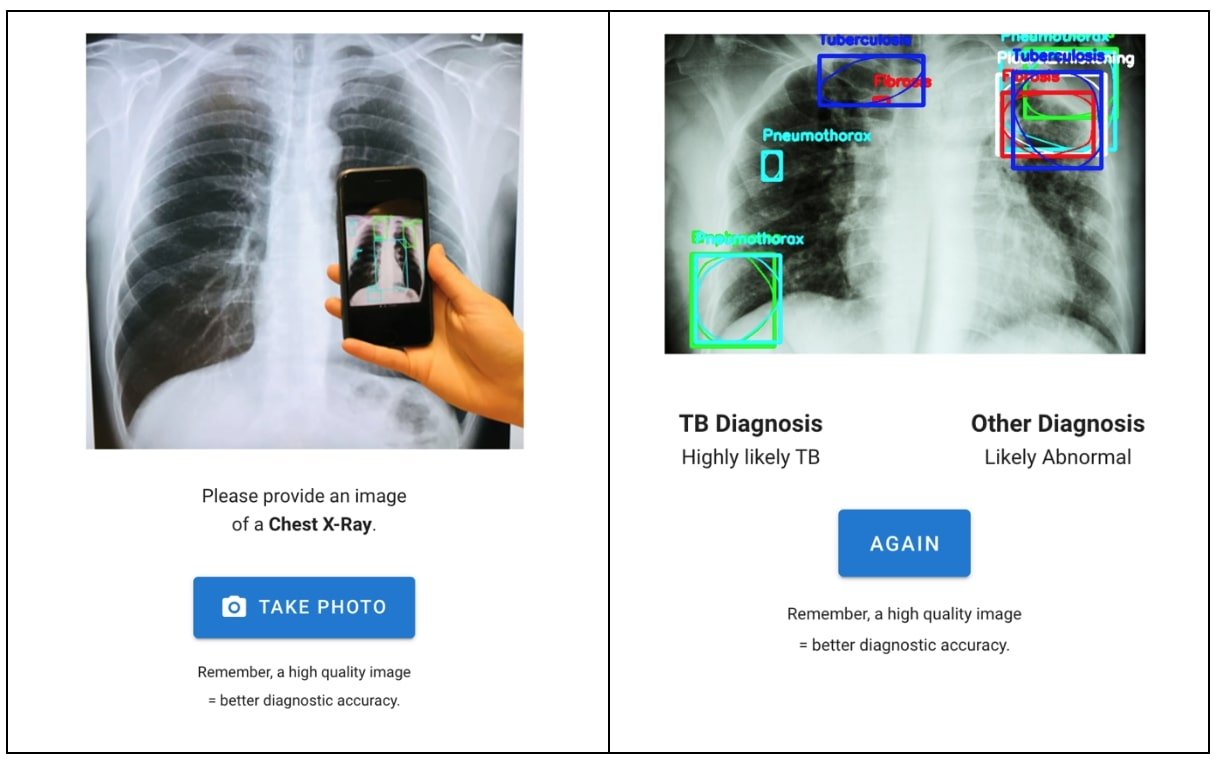
\includegraphics[width=0.8\linewidth]{pesti-report/images/epcon-web-app.jpg}
	\caption{EPCON demo web application}
	\label{fig:epcon-web-app}
\end{figure}

\\

This demo application had three main problems:

\begin{itemize}
\item
It connected directly with the artificial intelligence API, which made all the requests very slow
\item
It didn't use the latest symptoms payload they have added to the API
\item
It didn't persist data
\end{itemize}

So, our project was to build a system that would consume this machine learning API they have created that addressed all the listed problems and more.
\\ \\
EPCON wanted the app to be free to use for anyone, but they also wanted to have a registration system for doctors who wanted to persist all their screenings and patients. The app should allow doctors to manage patients and screen their respective X-rays.

\section{Functional requirements}

One of our first approaches during the first meeting was to try to define user-stories and write all of them down.

\\ \\
\begin{figure}[H]
	\centering
	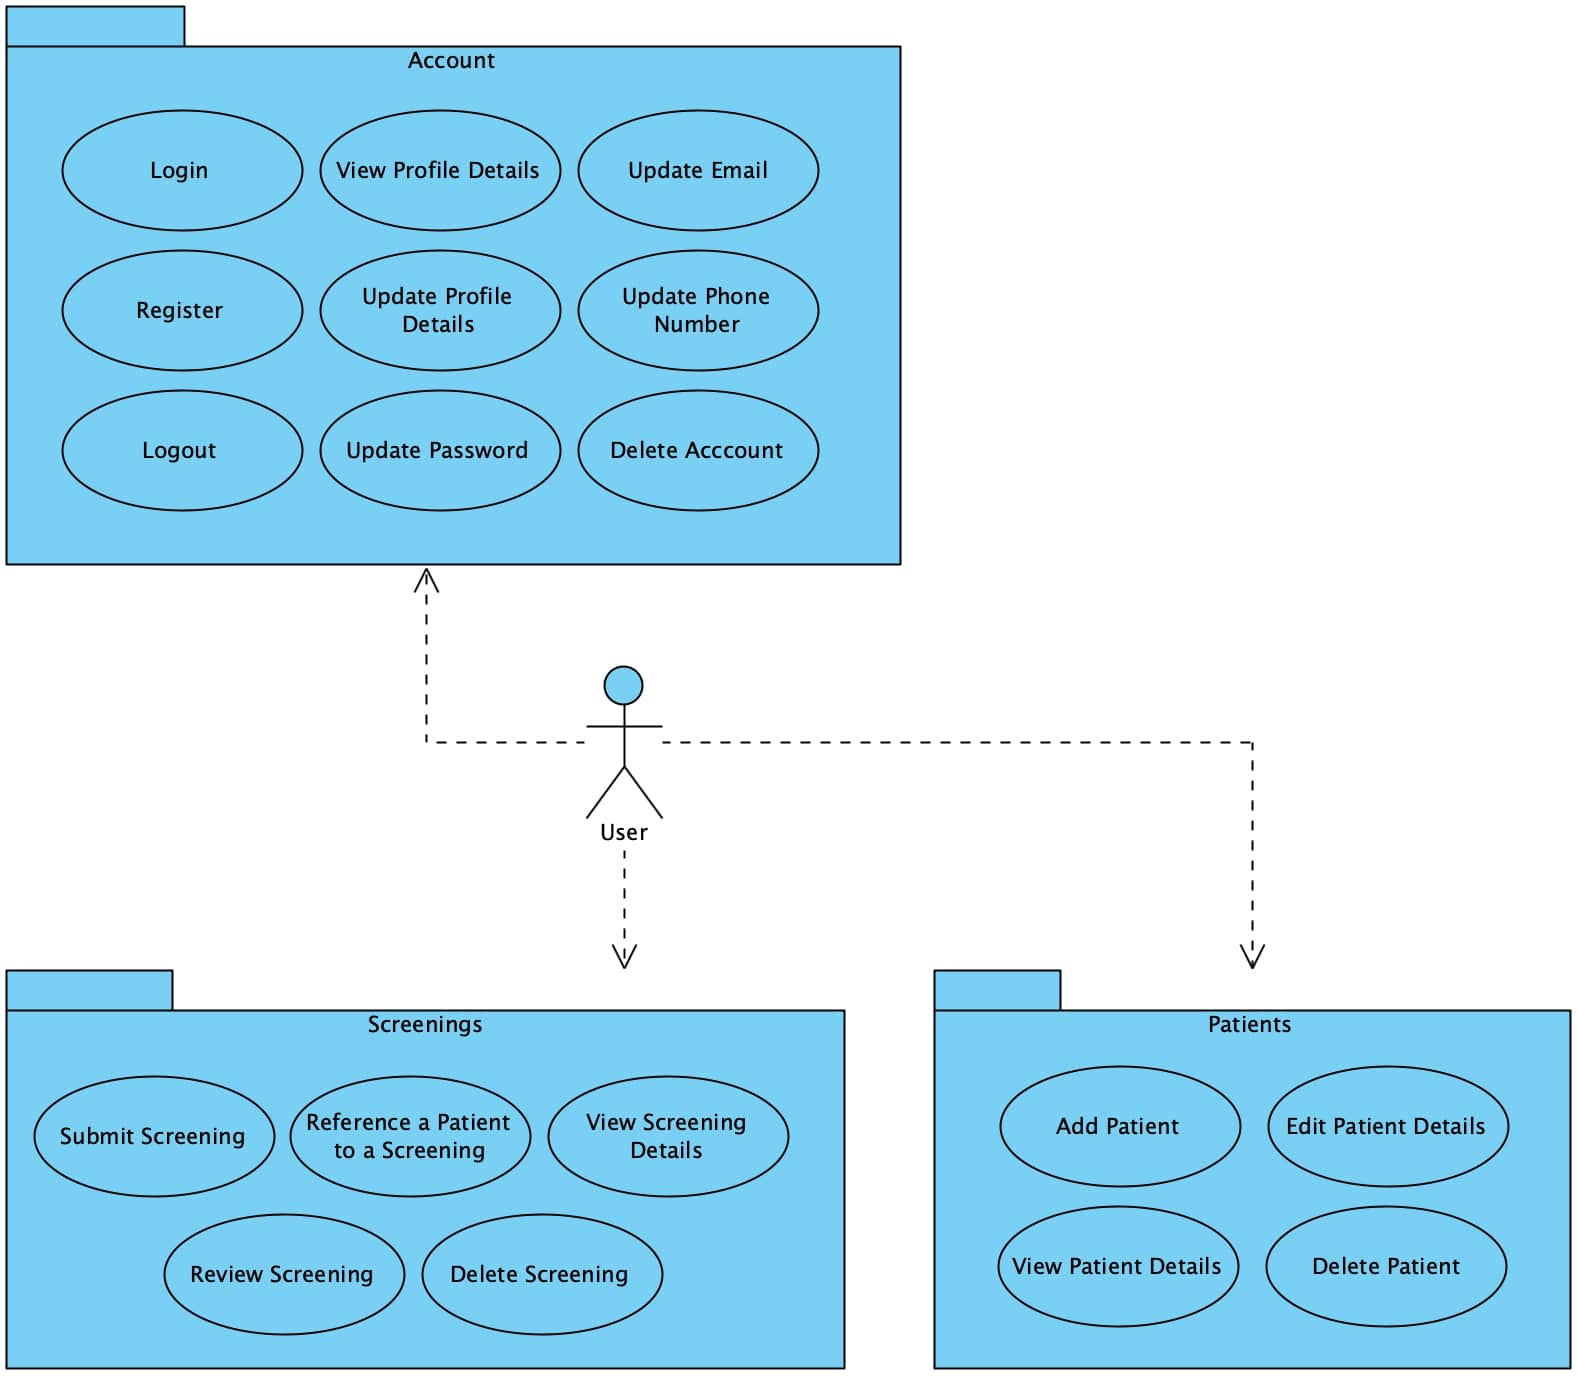
\includegraphics[width=1.0\linewidth]{pesti-report/images/use-case-diagram.jpg}
	\caption{Use case diagram}
	\label{fig:use-case-diagram}
\end{figure}

\\
Here are the use cases we collected:

\begin{itemize}
\item
A user can register using email, password and phone number
\item
A user can login using email and password
\item
A logged user can logout
\item
A logged user can view his/her profile
\item
A logged user can edit his/her profile (name, city, country and bio)
\item
A logged user can edit his/her password
\item
A logged user can edit his/her phone number
\item
A logged user can edit his/her email address
\item
A logged user can delete his/her account
\item
A user can submit a screening for diagnosis
\item
A user can view the diagnosis of a specific screening
\item
A user can view the list of his/her screenings
\item
A user can review a diagnosed screening
\item
A user can delete a specific screening
\item
A logged user can add a patient
\item
A logged user can view the list of his/her patients
\item
A logged user can view a specific patient details
\item
A logged user can edit a patient details(name, sex and year of birth)
\item
A logged user can delete a specific patient
\item
A logged user can reference a patient when submitting a screening
\item
A user can read the version changelog
\item
A user can read the about statement
\item
A user can read the terms and conditions
\item
A user can read the privacy policy
\item
A user can read the cookie policy
\end{itemize}

\section{Domain modeling}

The first step was to identify the different domains we would be working with. This was a time-consuming process because all of us were completely new to this computer-aided diagnosis area and also because all of us came from different countries and were speaking a non-native language. Nevertheless, we came up with these three different domains:

\begin{itemize}
\item
User
\item
Patient
\item
Screening
\end{itemize}

A \textbf{user} is anyone who is using the app. The app is targeted to be use by doctors, healthcare professionals or medical students, but it is free and open to anyone, so we thought it would be better to abstract from the concept of doctor.
\\ \\
A \textbf{patient} is a record added and persisted by a user and can be referenced on a screening.
\\ \\
A \textbf{screening} is an attempt to diagnose an X-ray pulmonary image.


\\ \\
\begin{figure}[!h]
	\centering
	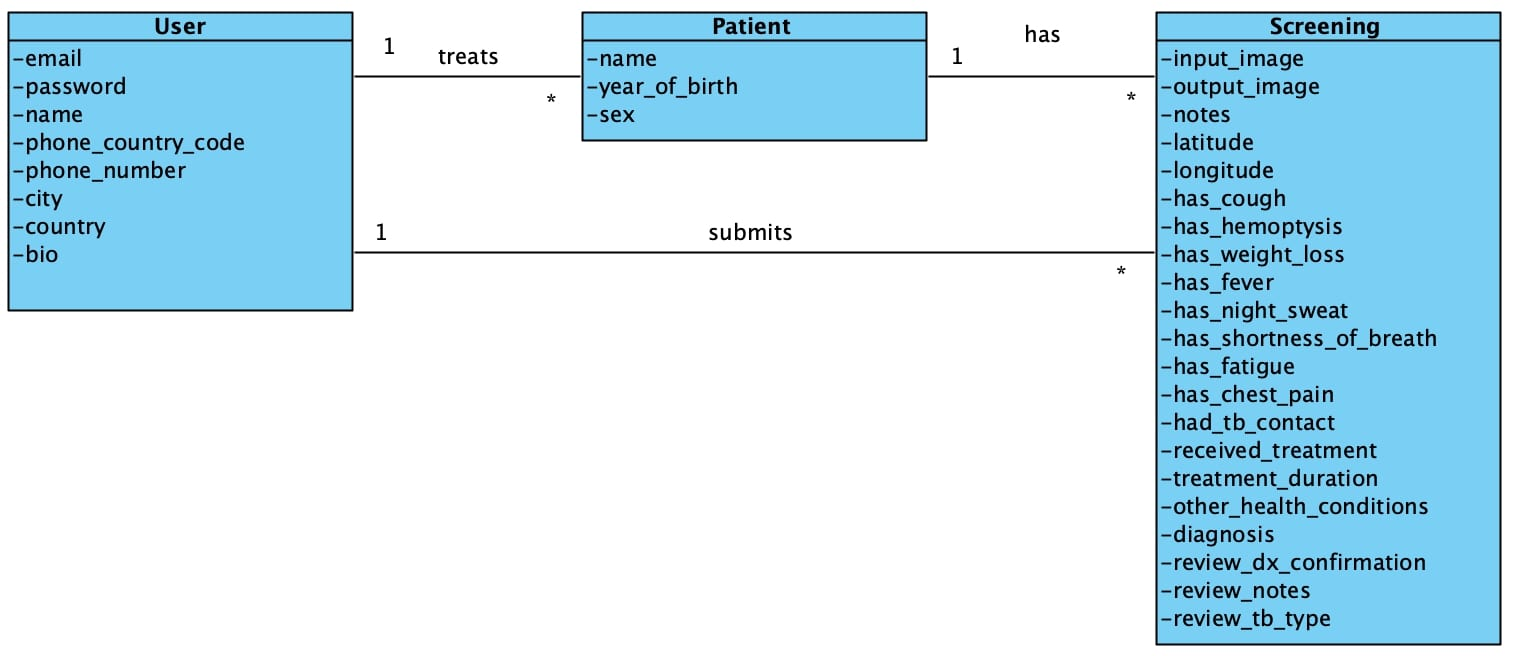
\includegraphics[width=1.0\linewidth]{pesti-report/images/domain-model.jpg}
	\caption{Domain model}
	\label{fig:domain-model}
\end{figure}
\\

\newpage\cleardoublepage

\chapter{Solution development}
\label{cap:solution-development}
% !TEX encoding = UTF-8 Unicode

EPCON had an already built API which provided computer-aided diagnostics. This API accepted an x-ray photo encoded using base 64 and returned a diagnosis estimation. This is a computer-intensive process and it usually took between 10 to 40 seconds to respond. The point was to create a backend RESTful API to hide complexity and manage those heavy requests and then develop clients that would connect to this facade API.
\\ \\
This new API would also deliver features that were not present on the EPCON API, like user authentication, patient and screening data storage.

\\ \\
\begin{figure}[H]
	\centering
	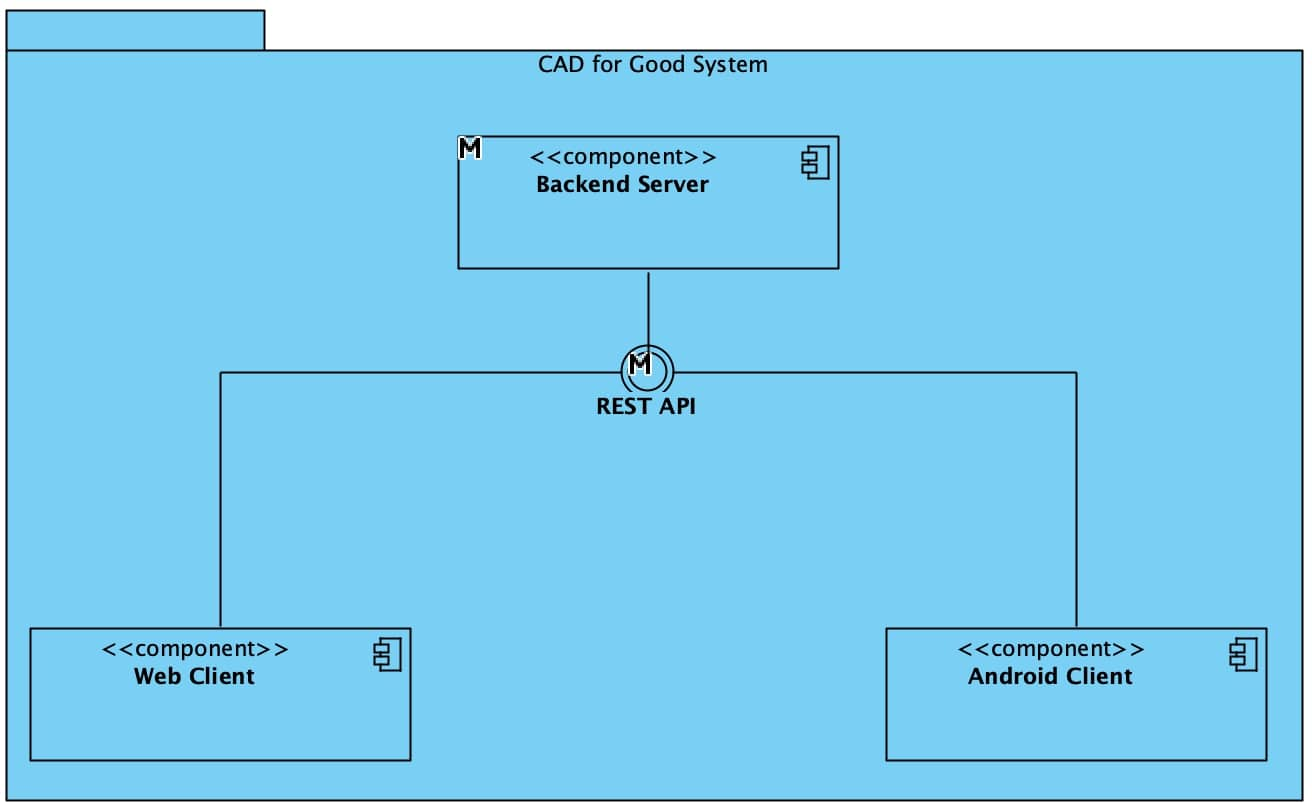
\includegraphics[width=1.0\linewidth]{pesti-report/images/global-system.jpg}
	\caption{System architecture}
	\label{fig:global-system}
\end{figure}
\\

The objective was to build clients with a focus on user-experience and which felt faster than directly requesting the EPCON servers.

\section{Implementation description}

To decide which technologies and frameworks we would use in order to develop the whole system we started by gathering information about the technical skills and previous experiences each of us had. We strongly thought about it and tried to not be influenced by the framework hype that exists nowadays. Many times during software development people put too much emphasis on the technology rather than the solution. We all agreed that we would go with the technologies that we felt comfortable with and not the ones that seemed better.
\\ \\
After this information gathering we decided to go with Node.js and Express for the back-end API, JavaScript and React for the web client and Kotlin and Java for the Android client.
\\
For designing the database schema we had to make some interesting decisions. One of the use cases required that the diagnose screening feature worked for both registered and unregistered users. For unregistered users the screening feature needed to be somehow connected to the specific device but EPCON also wanted to have the screening data persisted. To achieve this we added a device hash attribute to the Screening on the database schema and on the clients (web and Andorid) we would generate a unique hash and send it to the API on every diagnose screening request. This way we could merge all the local device screening with the ones persisted when an unregistered user finally decided to register.

\\ \\
\begin{figure}[H]
	\centering
	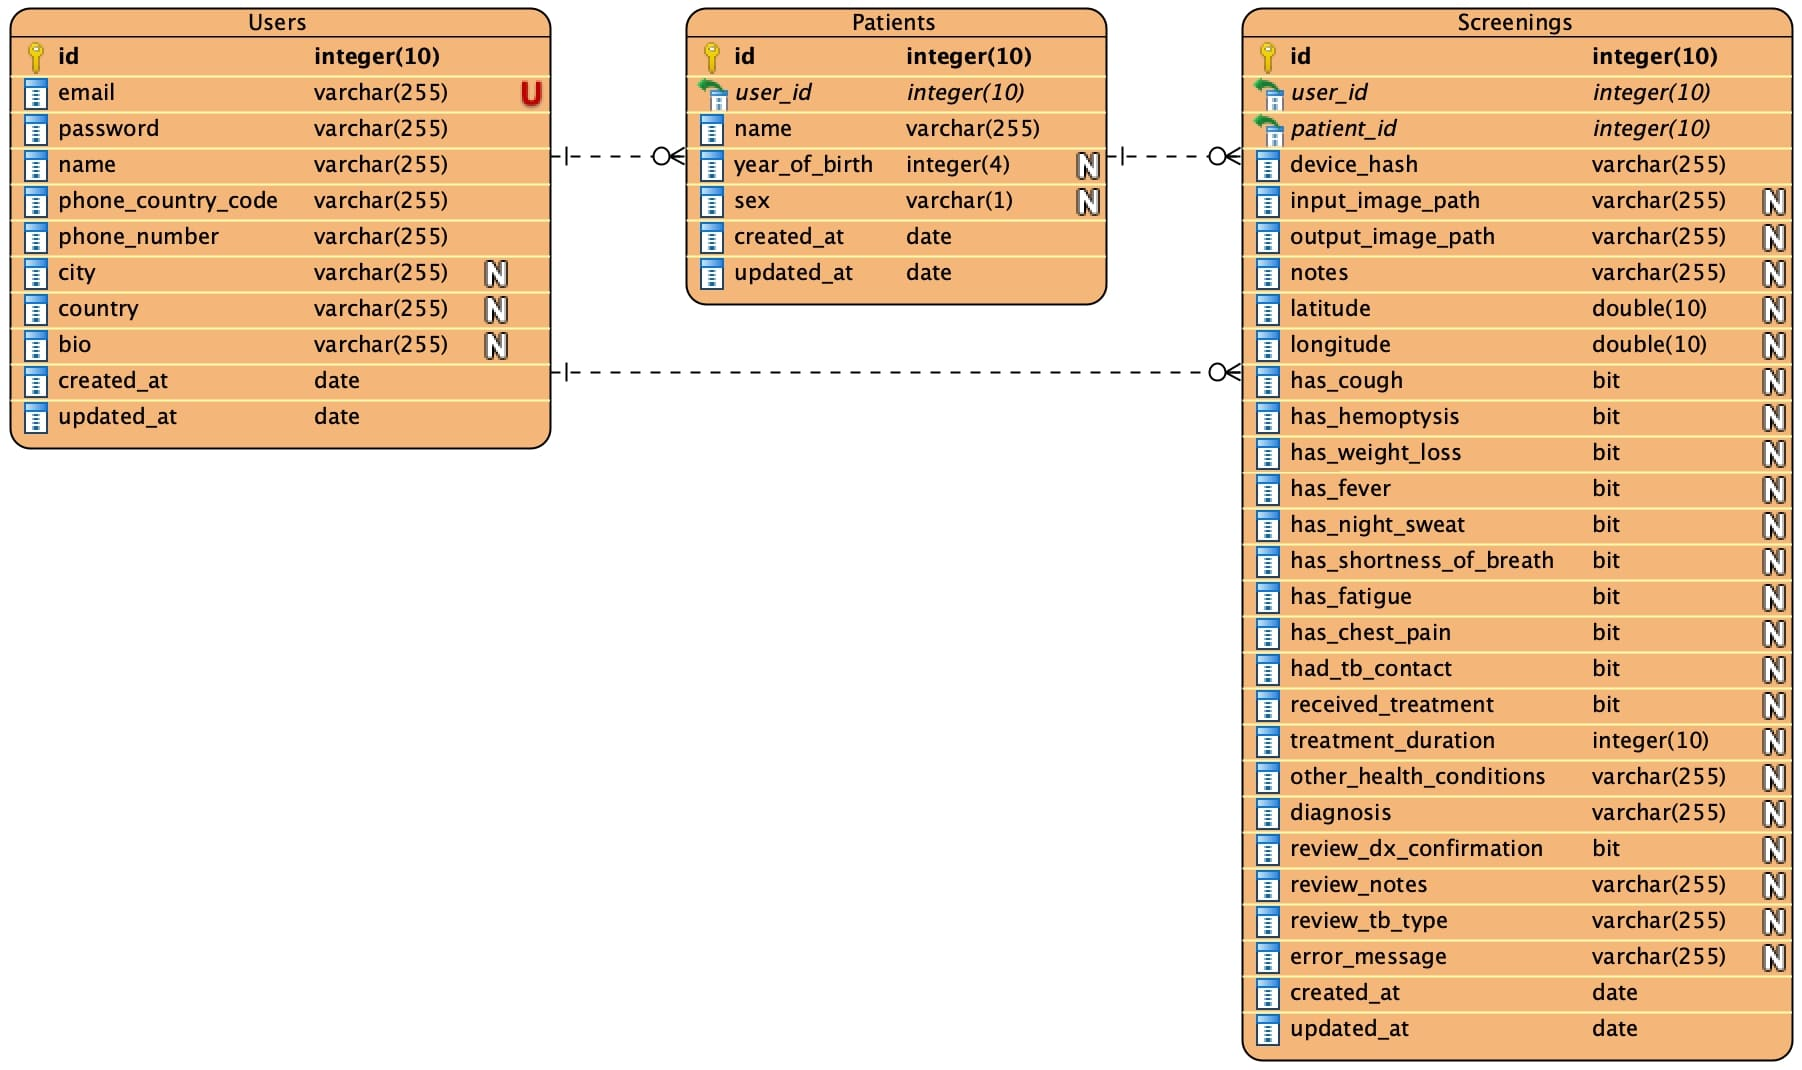
\includegraphics[width=1.0\linewidth]{pesti-report/images/database-schema.jpg}
	\caption{Database schema}
	\label{fig:database-schema}
\end{figure}
\\


\section{Backend architecture}

Our back-end was built using Node.js, a JavaScript run-time engine for server-side applications. To manage our API routes we used a popular Node.js framework named Express which made the endpoint development easier for us because of the framework API and nice online documentation.
\\ \\
We structured our code using different components that internally worked together. When a client would request our sever API the request would be caugth by our routes components, then it would pass by our middleware functions (different middlewares depending on the endpoint), then it would pass to our controllers and then, depending on the use case, hitting our database using our data access functions or generating some background service throught the use of events.


\\ \\
\begin{figure}[H]
	\centering
	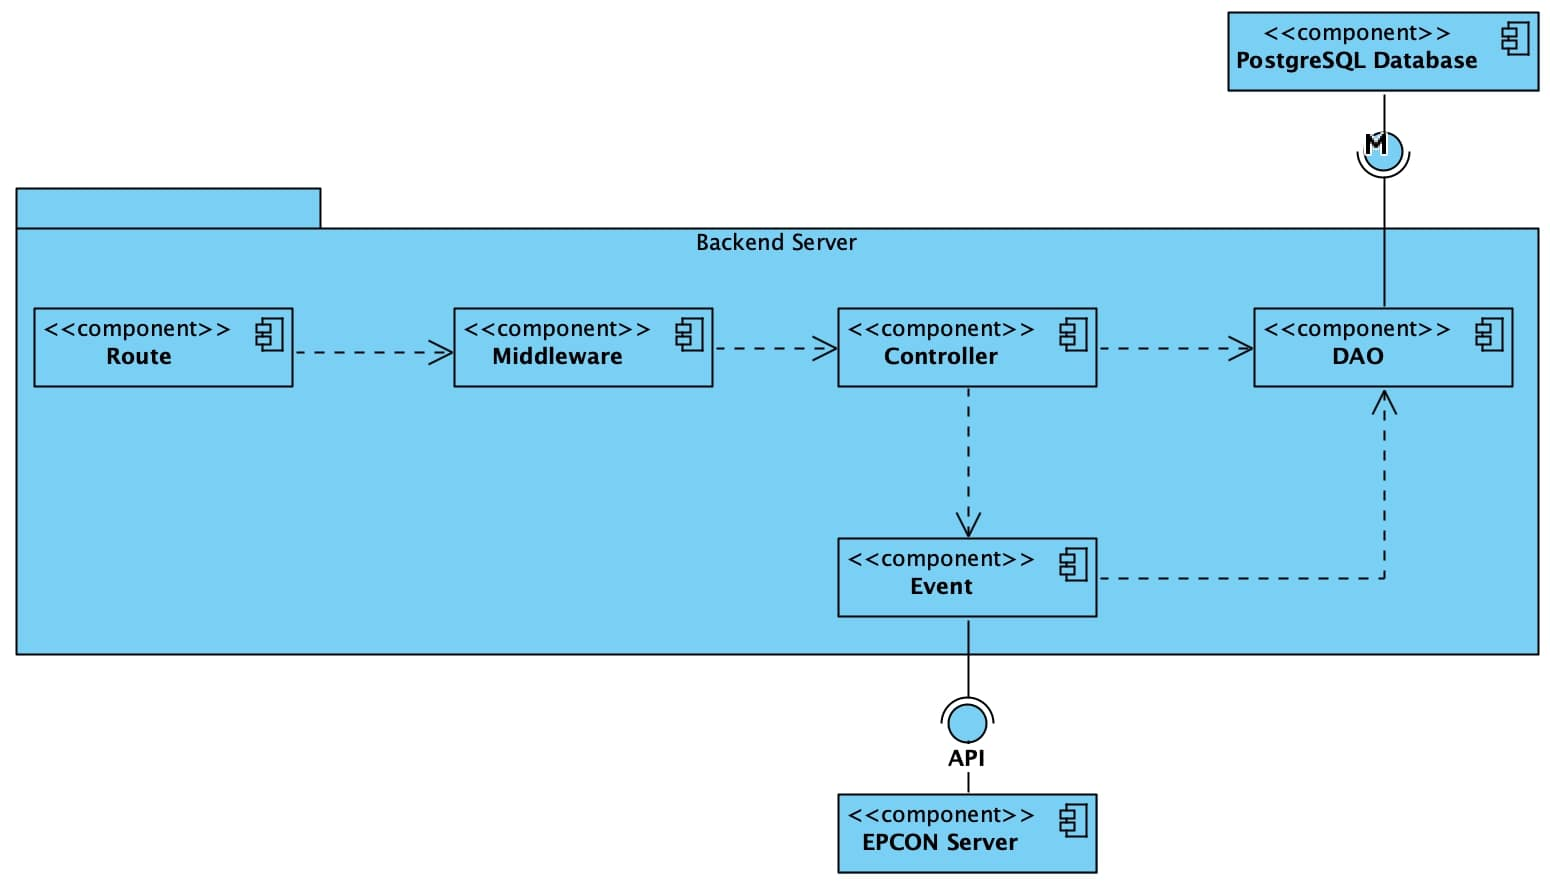
\includegraphics[width=1.0\linewidth]{pesti-report/images/backend-server-architecture.jpg}
	\caption{Backend server architecture}
	\label{fig:backend-server-architecture}
\end{figure}
\\

While designing and building this API, we had to make some interesting decisions. Here I will explain two of them in greater detail.

\subsection{User authentication}

To build our user authentication system with security on our minds we have created 2 different endpoints, one to register using email and password and another to login, also using email and password. When a user registers we check if the email address is already persisted in our database and if not we process to encrypt the password using a gold-standard open source password encryption npm module named bcrypt and then save the user on the database.
\\ \\
When the user logs in we compare the plain-text password to the encrypted one on the database using a bcrypt function and if it returns true we generate a JSON web token with the user id and return it to the client. Then client can decode the token but cannot modify it. This way, every time the client wants to request a private endpoint, it sends the token as a bearer token in the HTTP headers and the server can then decode the token, get the user id, and check if it was really that logged user who sent the request. This HTTP headers checking is done using our custom middleware functions.

\subsection{Background services}

One other challenge that we faced was the communication with EPCON API. To get diagnostics data from EPCON machine learning model, we have to first make a request to EPCON's authentication server, with a special username and login they provided for this project, get an authentication token (valid for 2 hours) from it, convert the multi-part-form JPEG or PNG image into base64 and then request an extremely slow-to-respond endpoint from EPCON bio-metrics server. This made the request to our endpoint extremely slow also, so we had to do it differently. When a user would submit a screening, it would save the initial details to the database and start a background service using a Node.js event. Then we would respond back to the client with the initial data stored about the screening, but with the diagnosis data still empty. And then, in the background service we would request the EPCON authentication server, get the token and then convert the images and request the bio-metrics server to get the diagnosis data. After that we would update that specific screening on the database.
\\ \\
After we updated the screening on the database we were thinking about using web-scokets to inform the user that the screening was updated with the diagnosis data, but, because of our lack of time, we did't yet implement this feature, so right now, we show the user information that says the screening is still processing and ask the user to refresh the page to fetch new data. We use this short polling technique while we don't have this web-socket feature proper implemented yet.


\section{Web client structure}

Our web application was written using JavaScript and React. We boostrapped our project using create-react-app which is a command line tool built by Facebook to people set up a modern React web app \cite{CreateReactApp}, and Bootstrap which is the world’s most popular front-end open source framework to quickly design and customize responsive mobile-first sites, featuring SASS variables and mixins, responsive grid system, extensive pre-built components, and powerful JavaScript plugins \cite{Bootstrap}.
\\ \\
The overall component schema of the web application can be seen in the image below.

\\ \\
\begin{figure}[H]
	\centering
	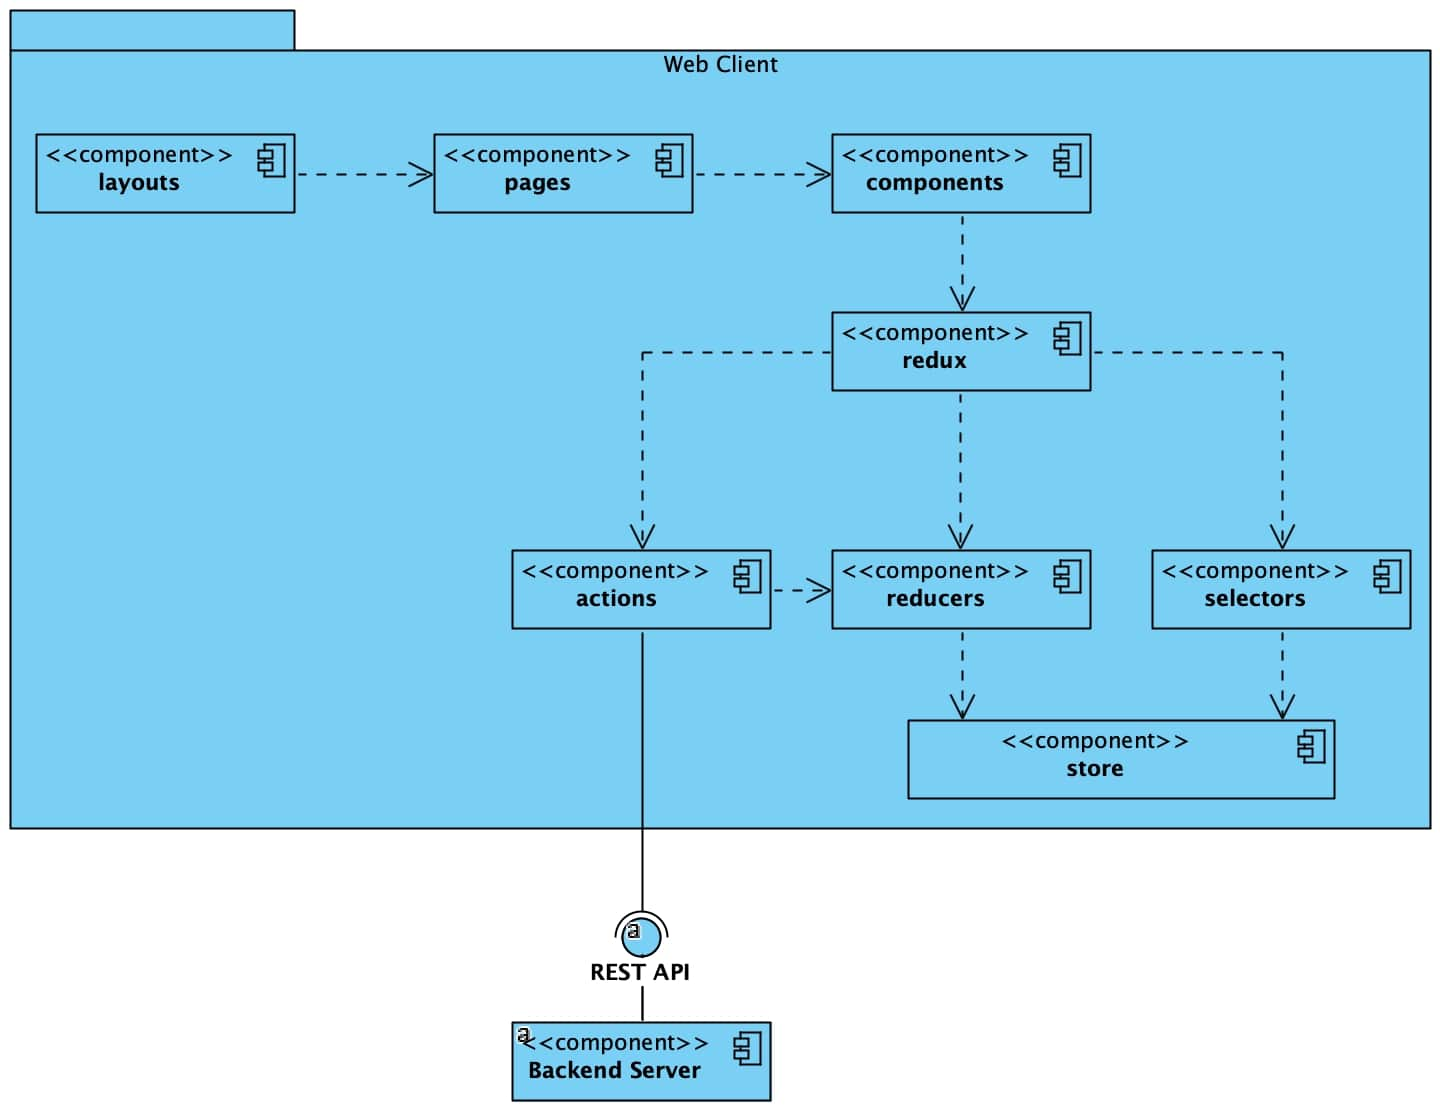
\includegraphics[width=1.0\linewidth]{pesti-report/images/web-client-structure.jpg}
	\caption{Web client structure}
	\label{fig:web-client-structure}
\end{figure}
\\

The visualization part is composed of pages, composed by a layout and many components.
\\ \\
If a component needs to post some data through the API of our backend server it needs to use our Redux layer. The component uses this layer by calling action functions, which are going to hit the API and call different action types which activate different reducers that will mutate the Redux store state.
\\ \\
If a component needs to fetch some data from the API it also needs to pass by the Redux layer, this time by using selector functions, which will return a specific piece of state to that component.
\\ \\
Below we can see a screenshot of our Redux store state at a given point in time. It holds information about the user profile, loading and error states and a memory cache of all the patients and screenings that were already fetched from the API.

\\ \\
\begin{figure}[H]
	\centering
	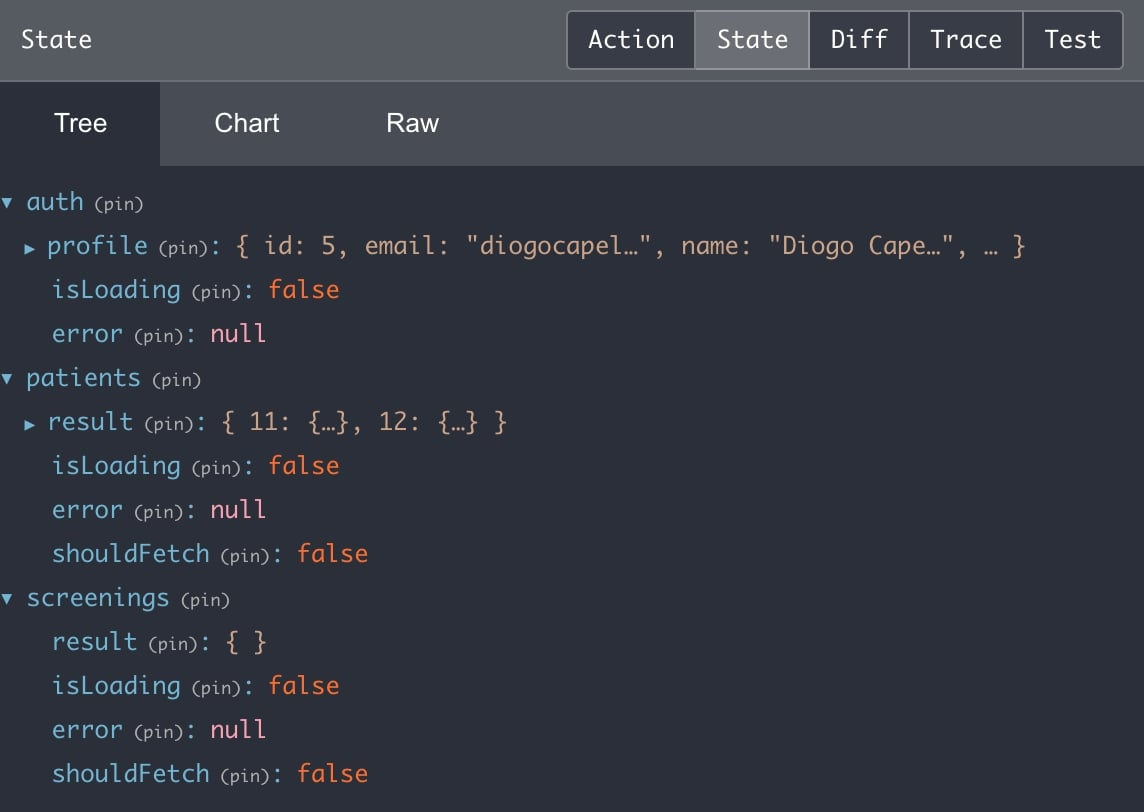
\includegraphics[width=1.0\linewidth]{pesti-report/images/redux-store.jpg}
	\caption{Redux store}
	\label{fig:redux-store}
\end{figure}
\\

To style the website to match EPCON design needs we decided to use a SCSS, a CSS tool that give us more options when writing styles for our layouts and components.
\\ \\
In the figure below we can see a screenshot of the homepage of the web application.

\\ \\
\begin{figure}[H]
	\centering
	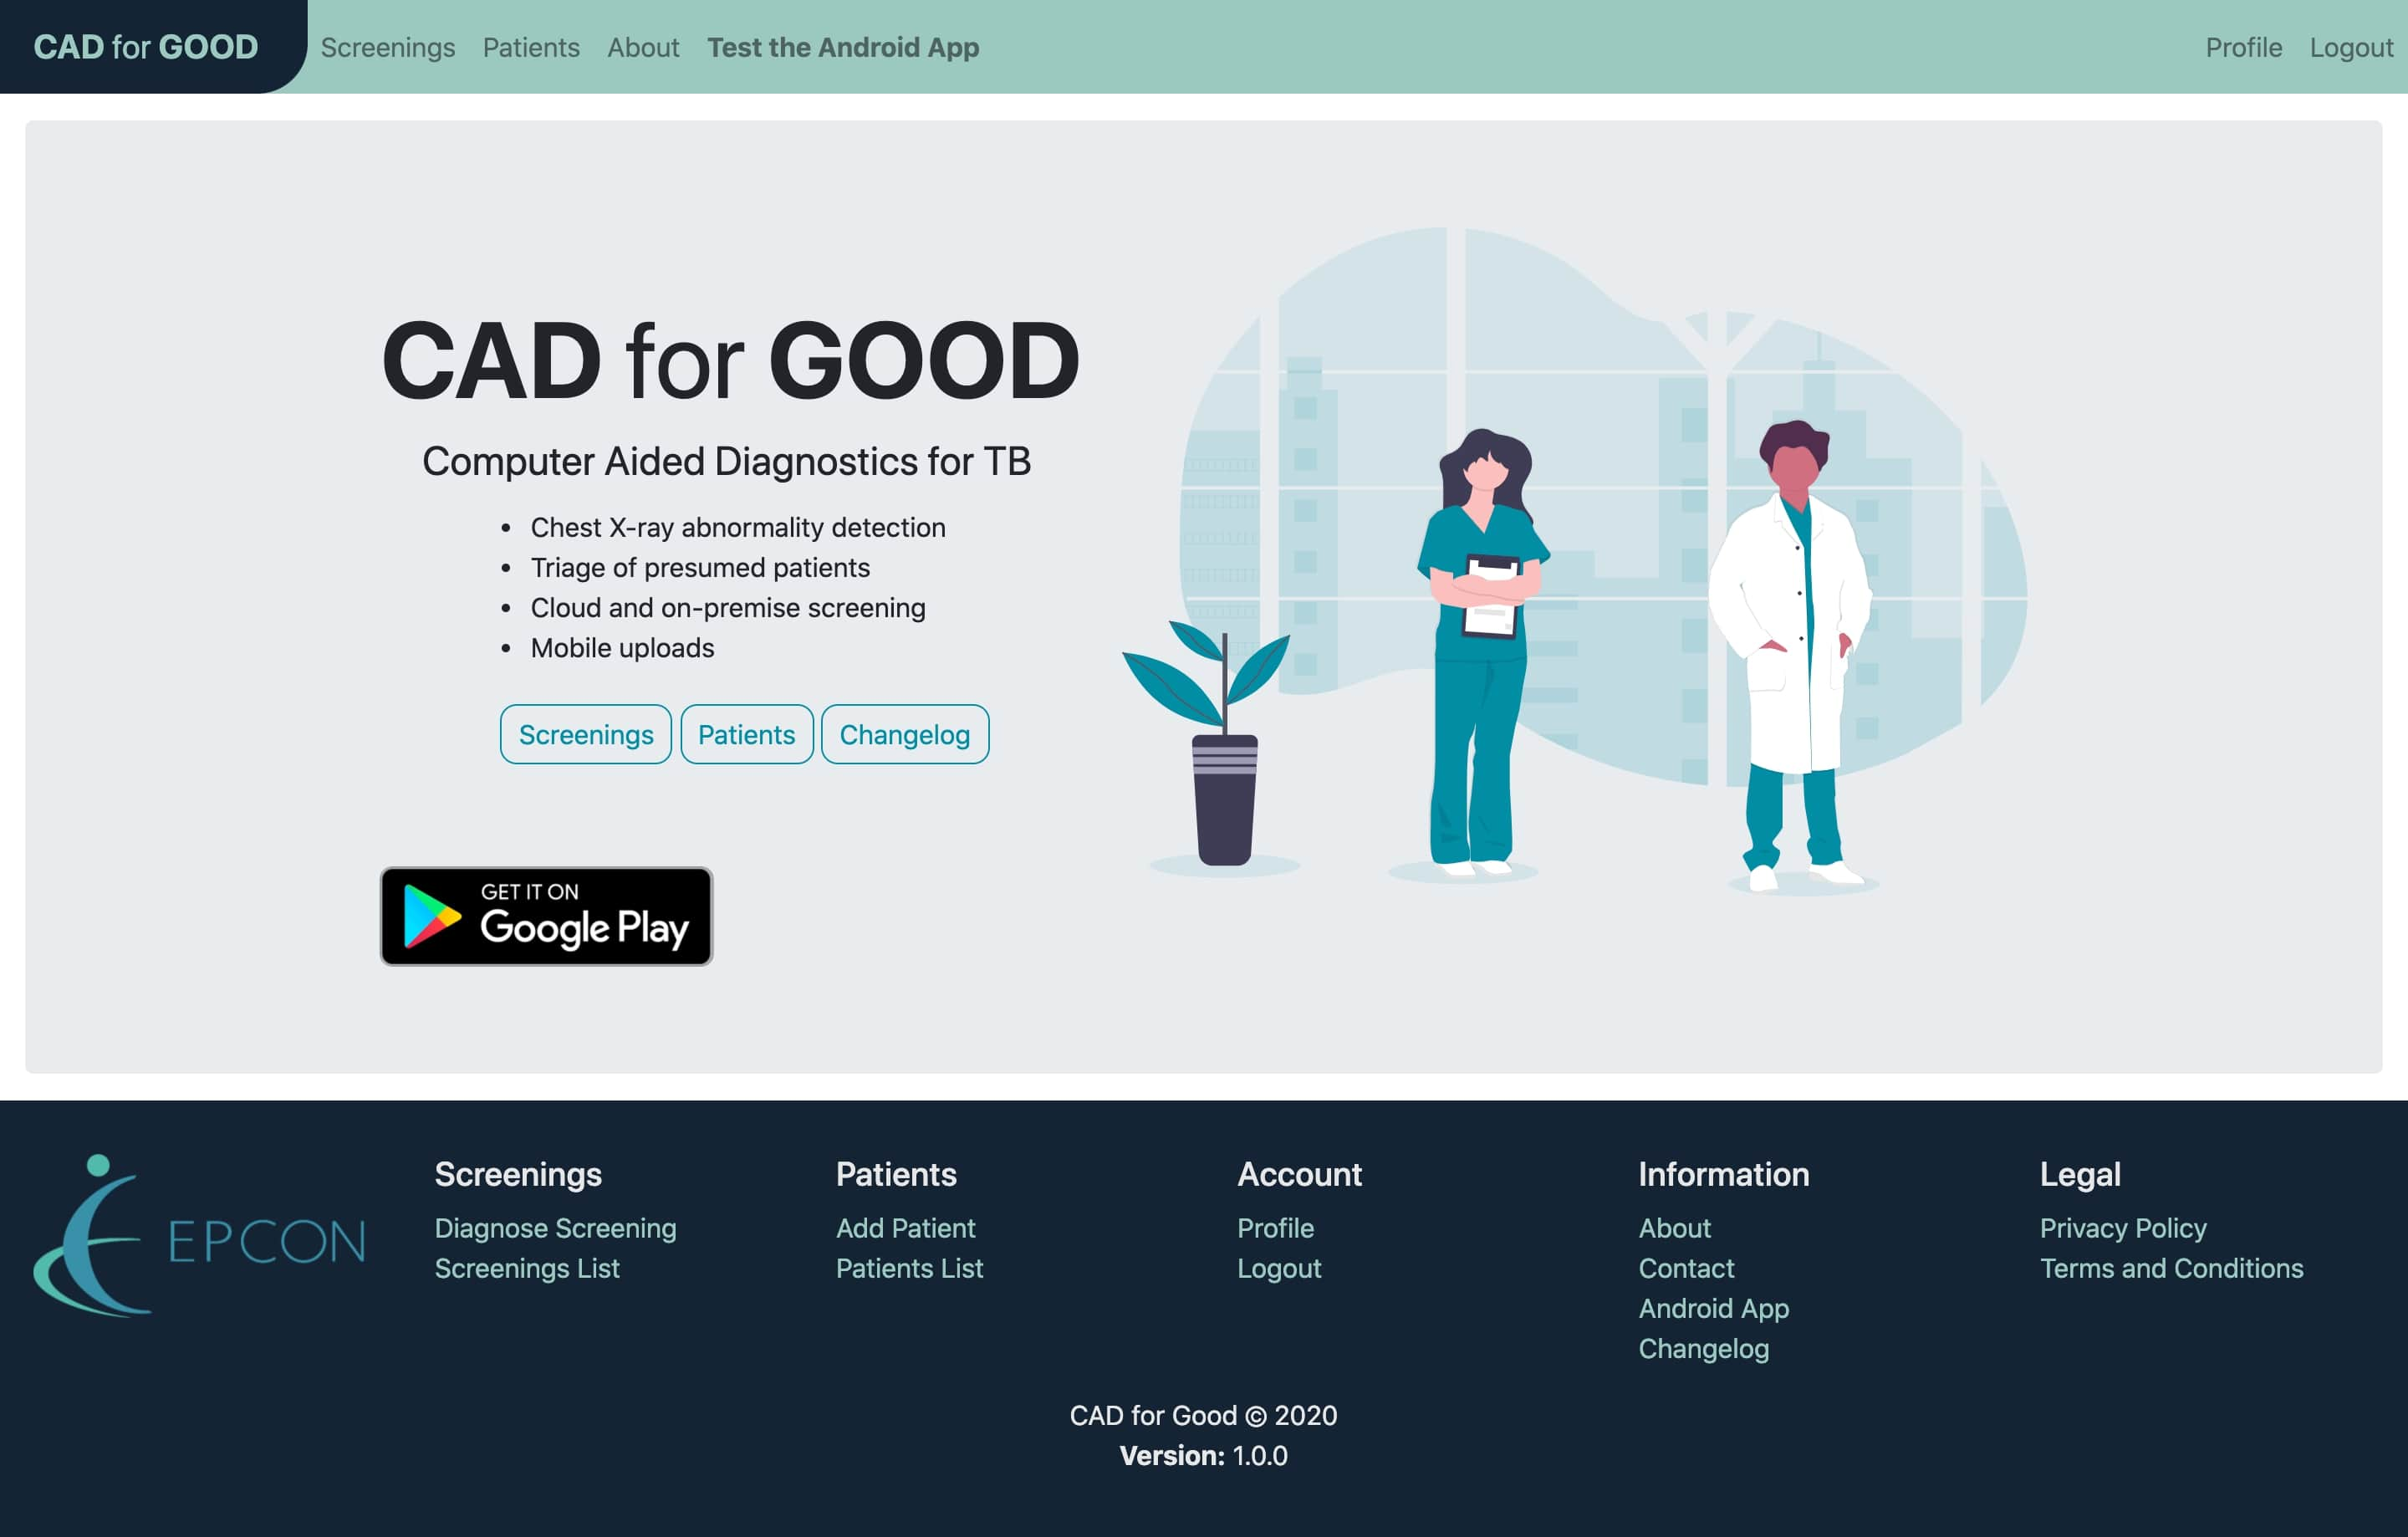
\includegraphics[width=1.0\linewidth]{pesti-report/images/web-client-screenshot-homepage.jpg}
	\caption{Homepage of the web application}
	\label{fig:web-client-screenshot-homepage}
\end{figure}
\\

The screening process starts by the client generating an unique device hash so every request do diagnose a screening can be traced back to the device.

\\ \\
\begin{figure}[H]
	\centering
	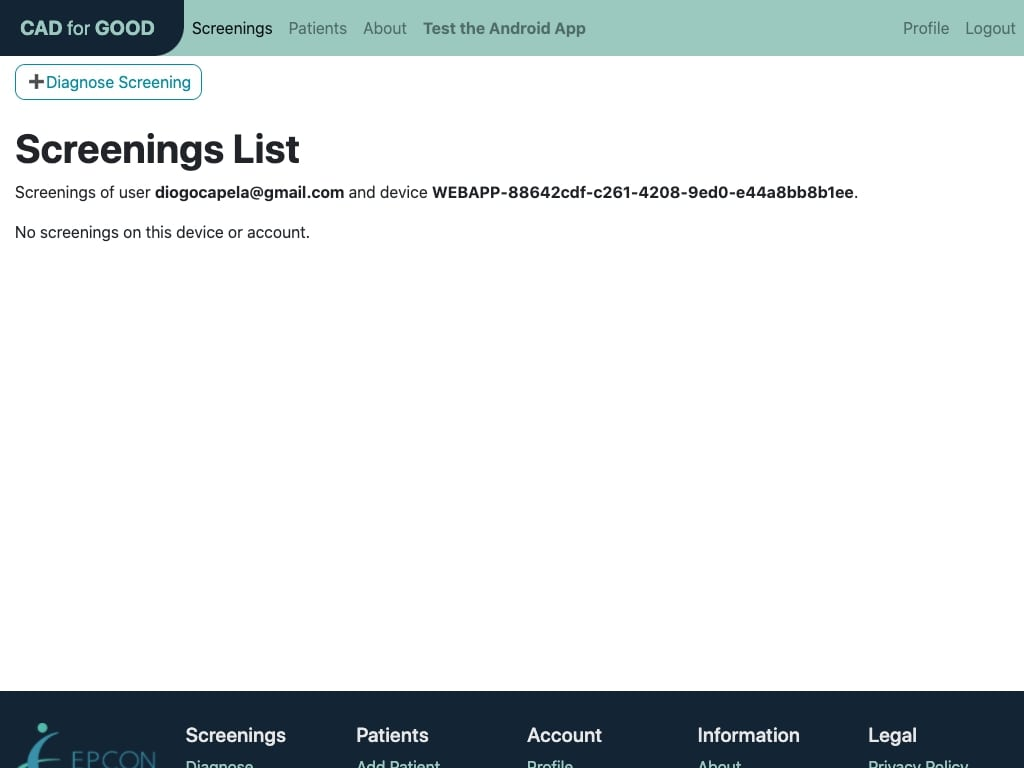
\includegraphics[width=1.0\linewidth]{pesti-report/images/web-client-screenshot-screenings-01.jpg}
	\caption{Empty screenings list}
	\label{fig:web-client-screenshot-screenings-01}
\end{figure}
\\

After we click on diagnose screening we are taken to a page where we can upload the X-ray picture and fill all the symptoms and additional details.

\\ \\
\begin{figure}[H]
	\centering
	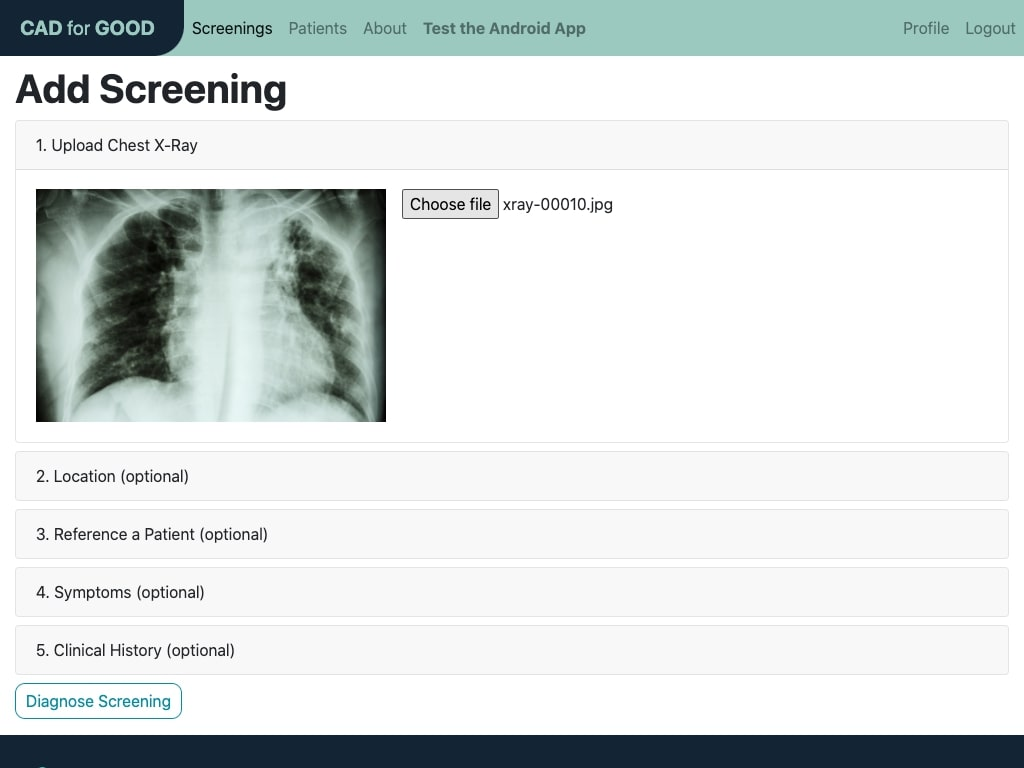
\includegraphics[width=1.0\linewidth]{pesti-report/images/web-client-screenshot-screenings-02.jpg}
	\caption{Submit a screening page}
	\label{fig:web-client-screenshot-screenings-02}
\end{figure}
\\

When we submit a screening the server is running it as a background service, so we should wait on the client side for it to be completed. After the screening has diagnostic data from the back-end we can view it in the screening details page you can see below:

\\ \\
\begin{figure}[H]
	\centering
	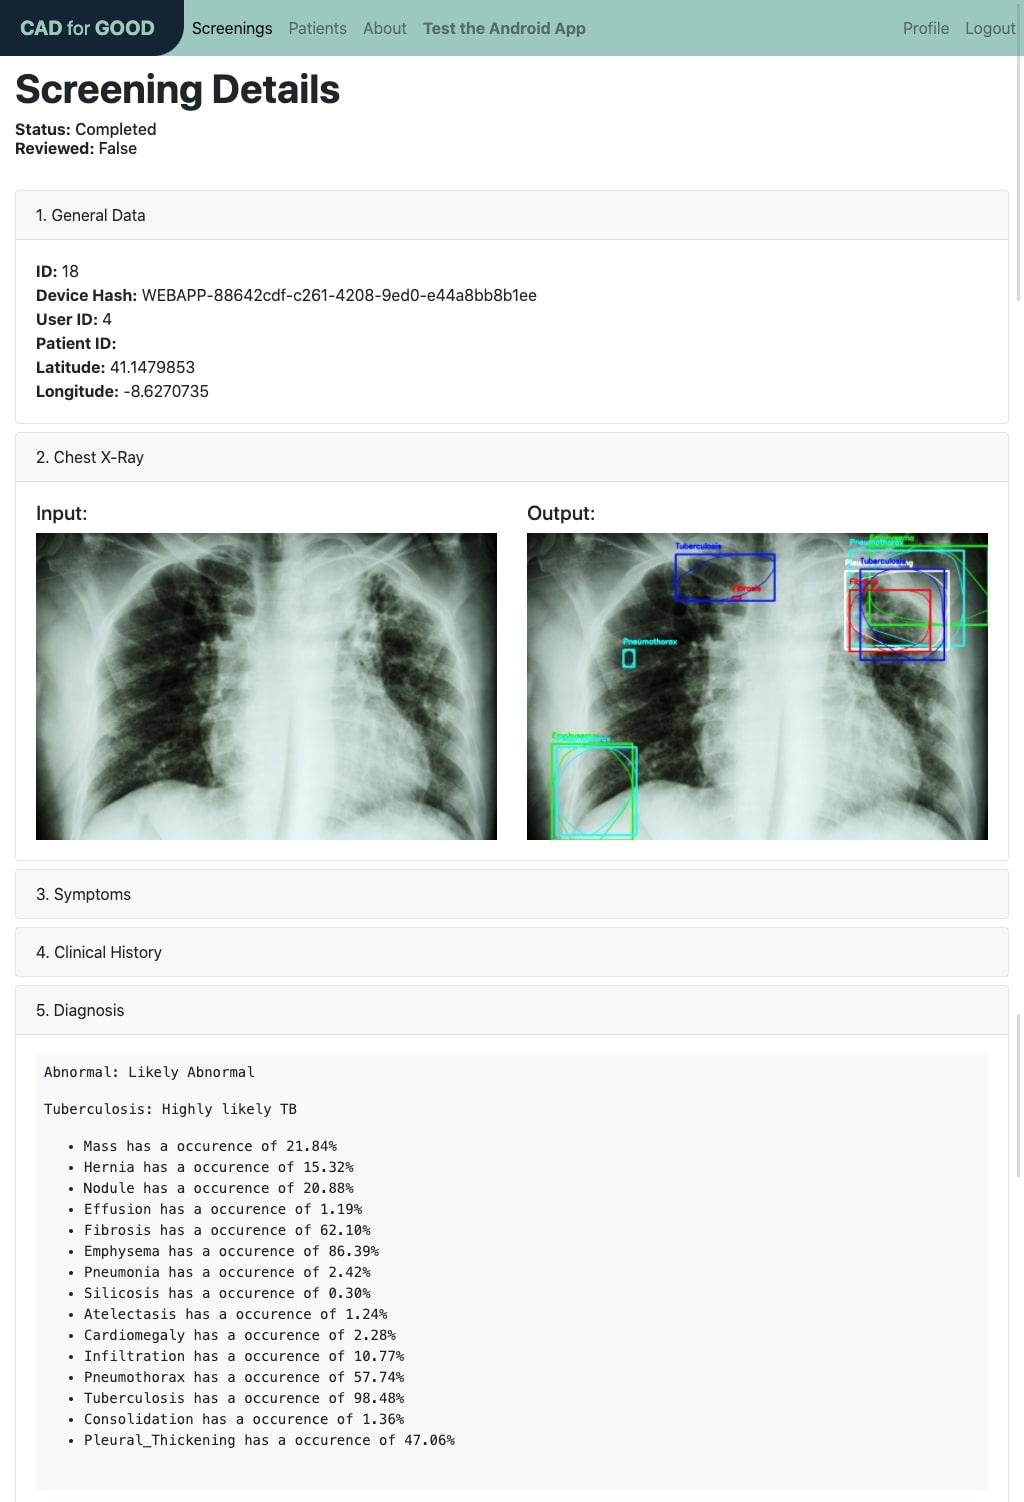
\includegraphics[width=1.0\linewidth]{pesti-report/images/web-client-screenshot-screenings-04.jpg}
	\caption{Screening details page}
	\label{fig:web-client-screenshot-screenings-04}
\end{figure}
\\



\section{Android client structure}

To build the Android client we use the standard development tools: Android Studio and the JDK for Android. We decided to build a native application because most of our team was familiar with Java, the programming language used by Android Studio and the Android API.
\\ \\
We divided our components into layouts, composed by activities and fragments, both of them with logic glued to the respective controllers. And then this controllers would connect to our repositories which saved data locally using a SQLite database, or communicated directly with out back-end API.

\\ \\
\begin{figure}[H]
	\centering
	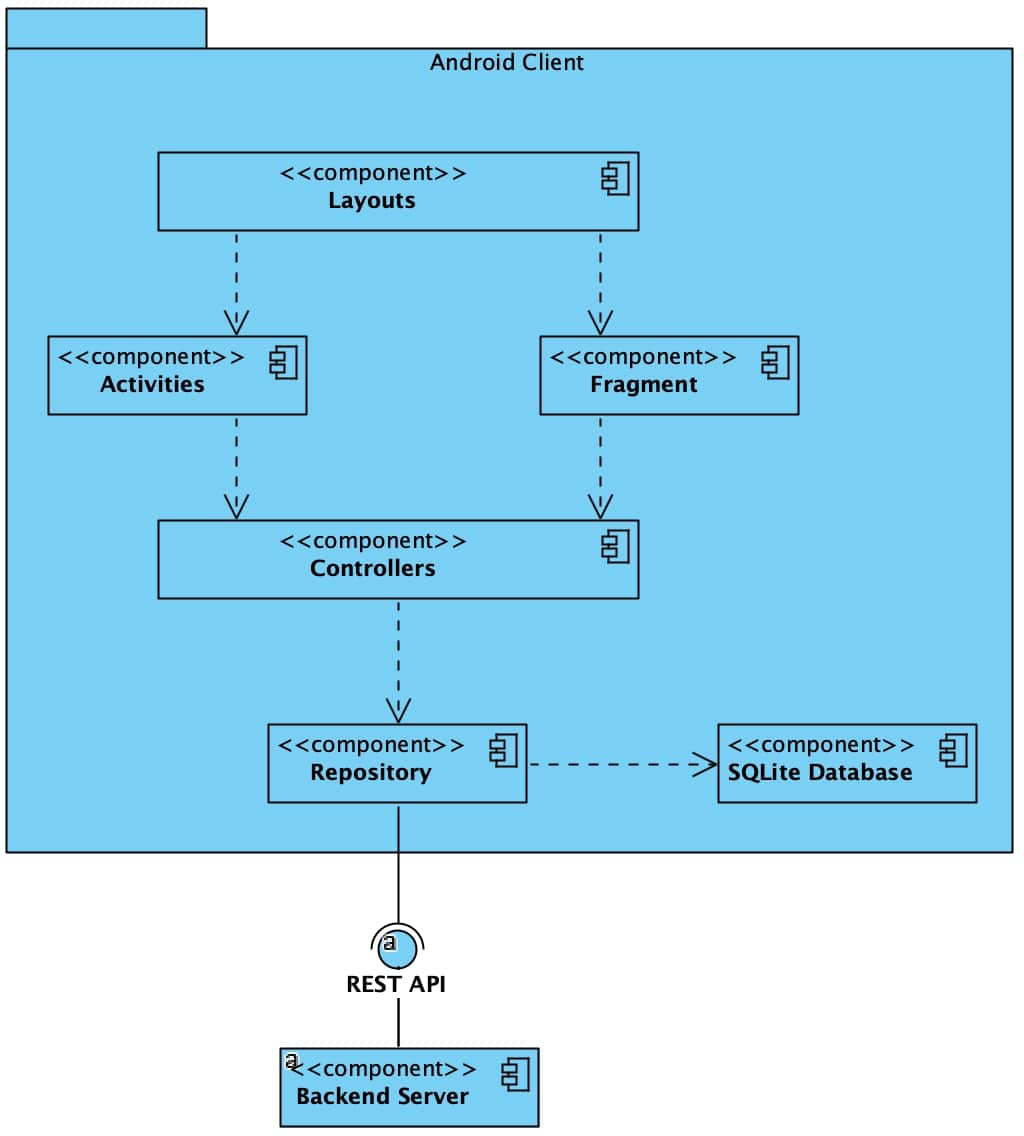
\includegraphics[width=1.0\linewidth]{pesti-report/images/android-client-structure.jpg}
	\caption{Android client structure}
	\label{fig:android-client-structure}
\end{figure}
\\

Below are some screenshots of the authentication layout we have at the time of this report.

\\ \\
\begin{figure}[H]
	\centering
	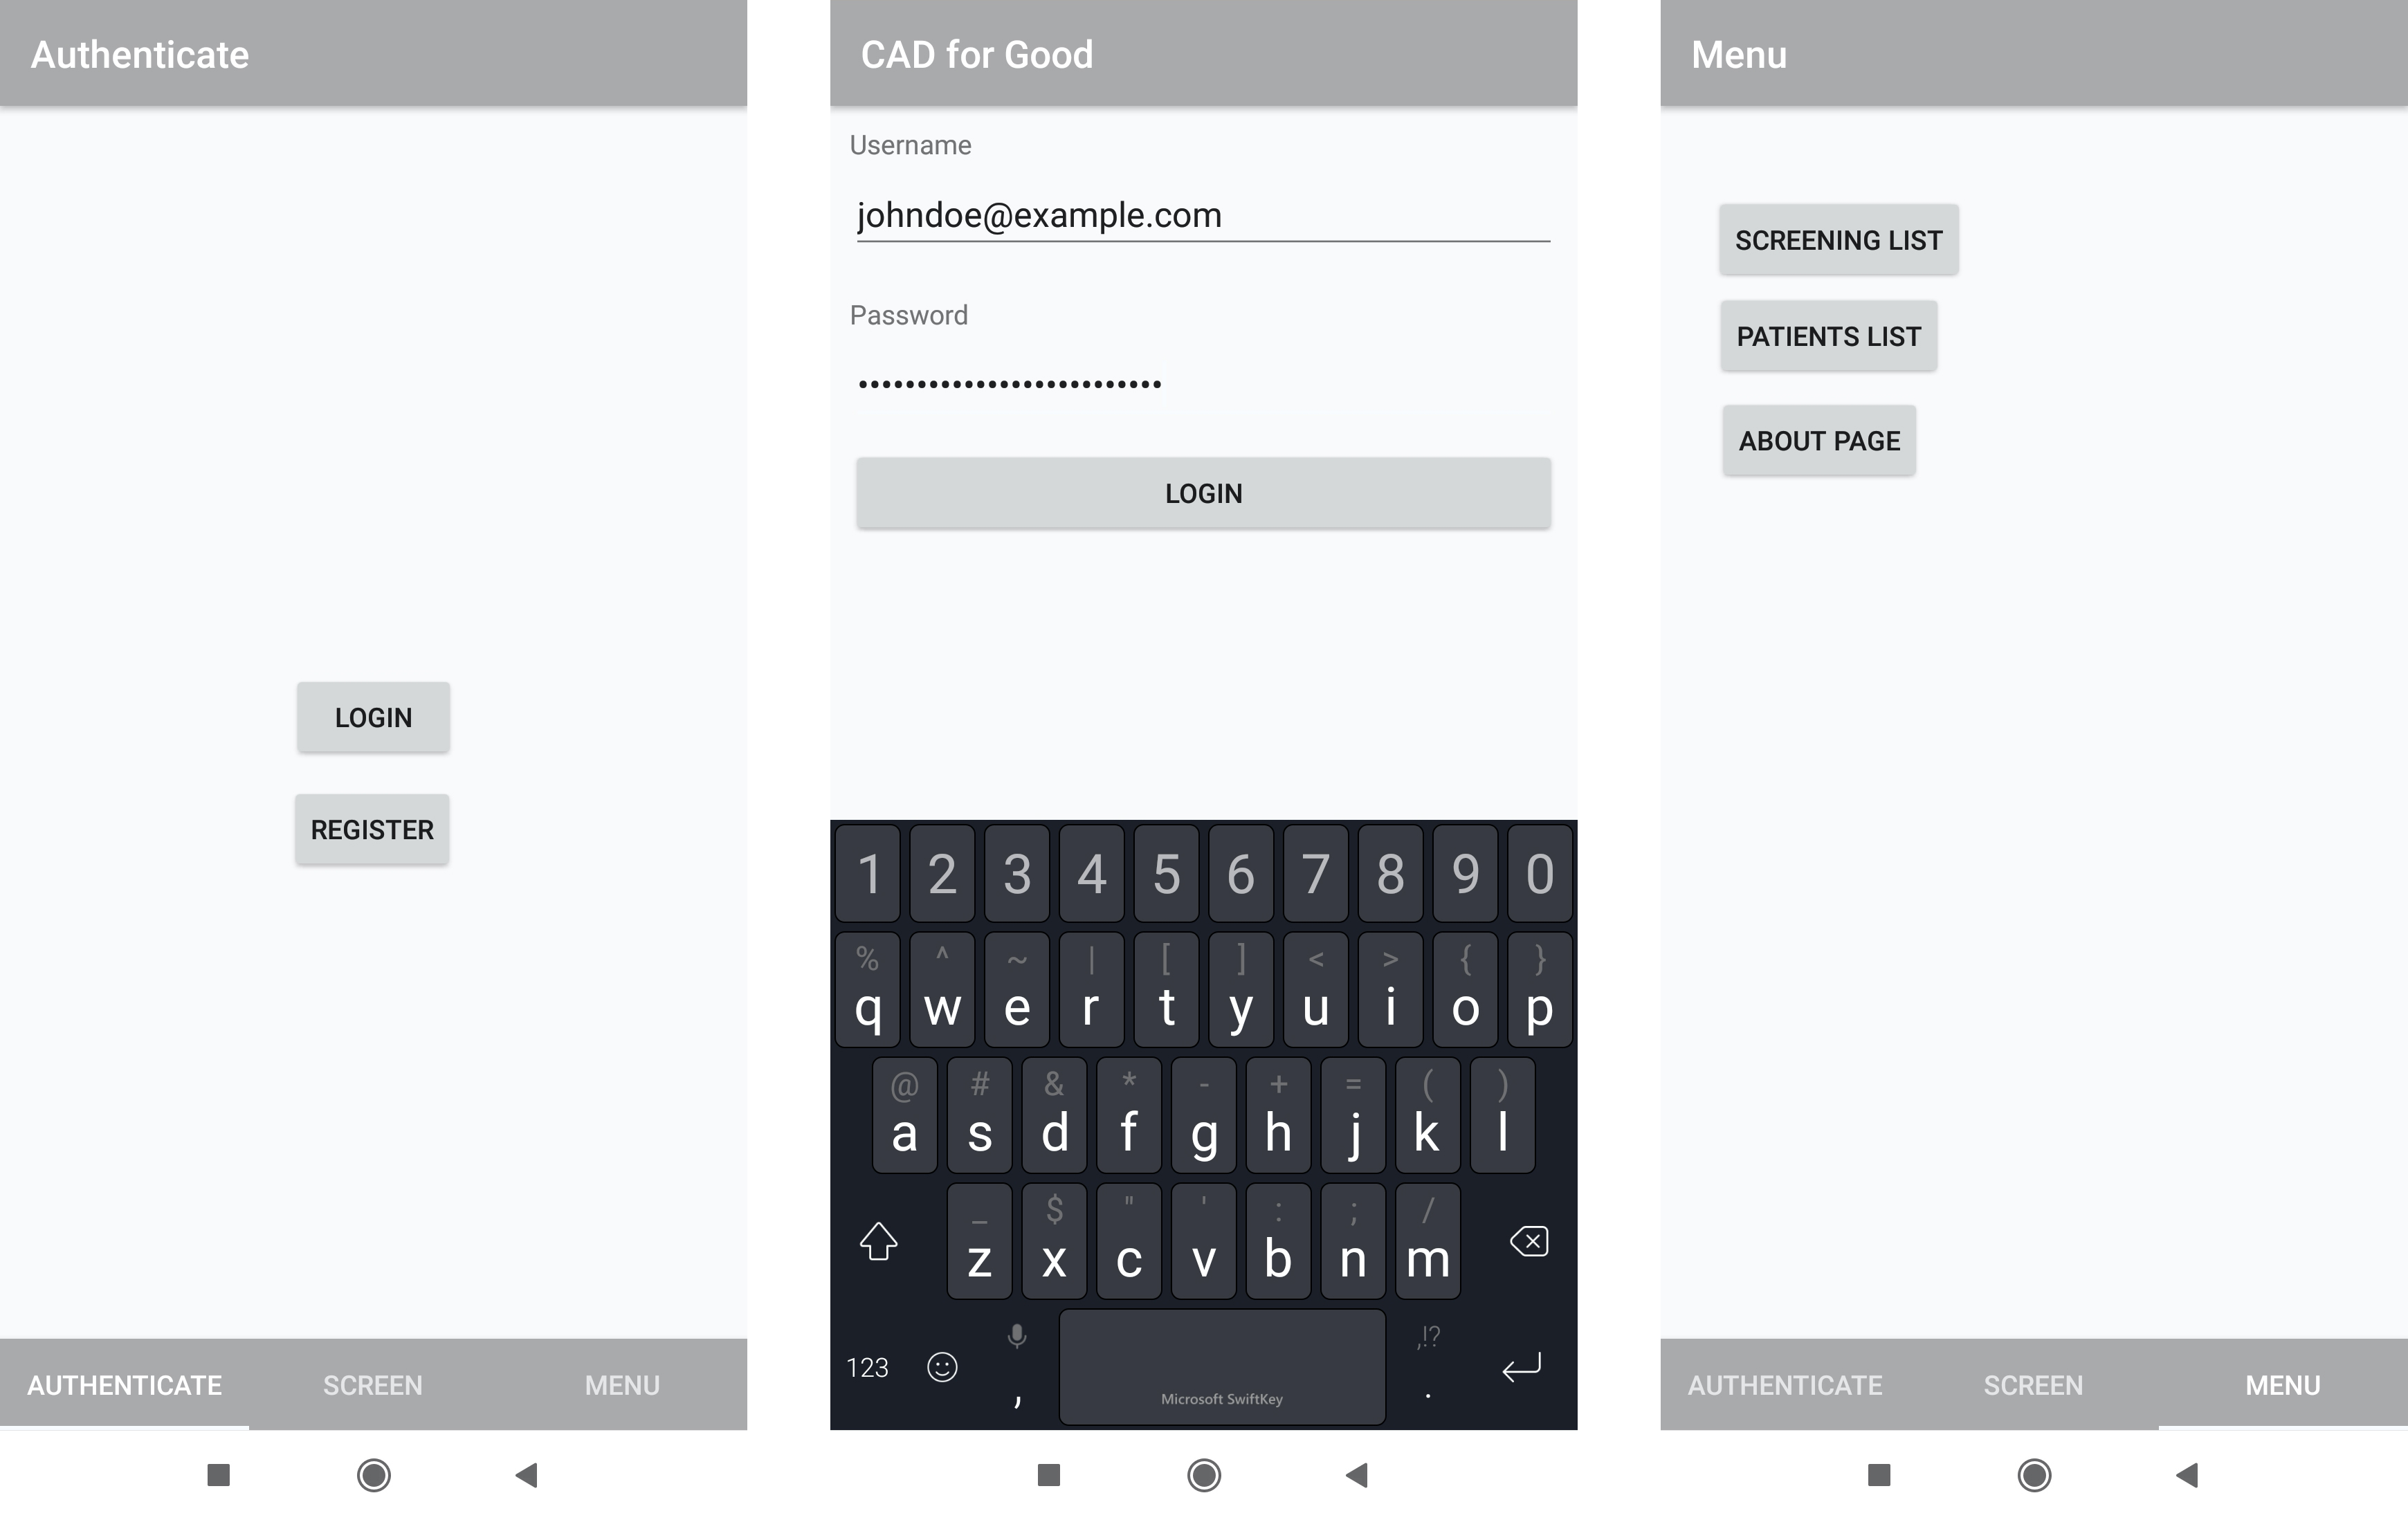
\includegraphics[width=1.0\linewidth]{pesti-report/images/android-client-screenshot-authentication.jpg}
	\caption{Android client authentication}
	\label{fig:android-client-authentication}
\end{figure}
\\

And below you can find the MVP layout for the screening submission process on our mobile app.

\\ \\
\begin{figure}[H]
	\centering
	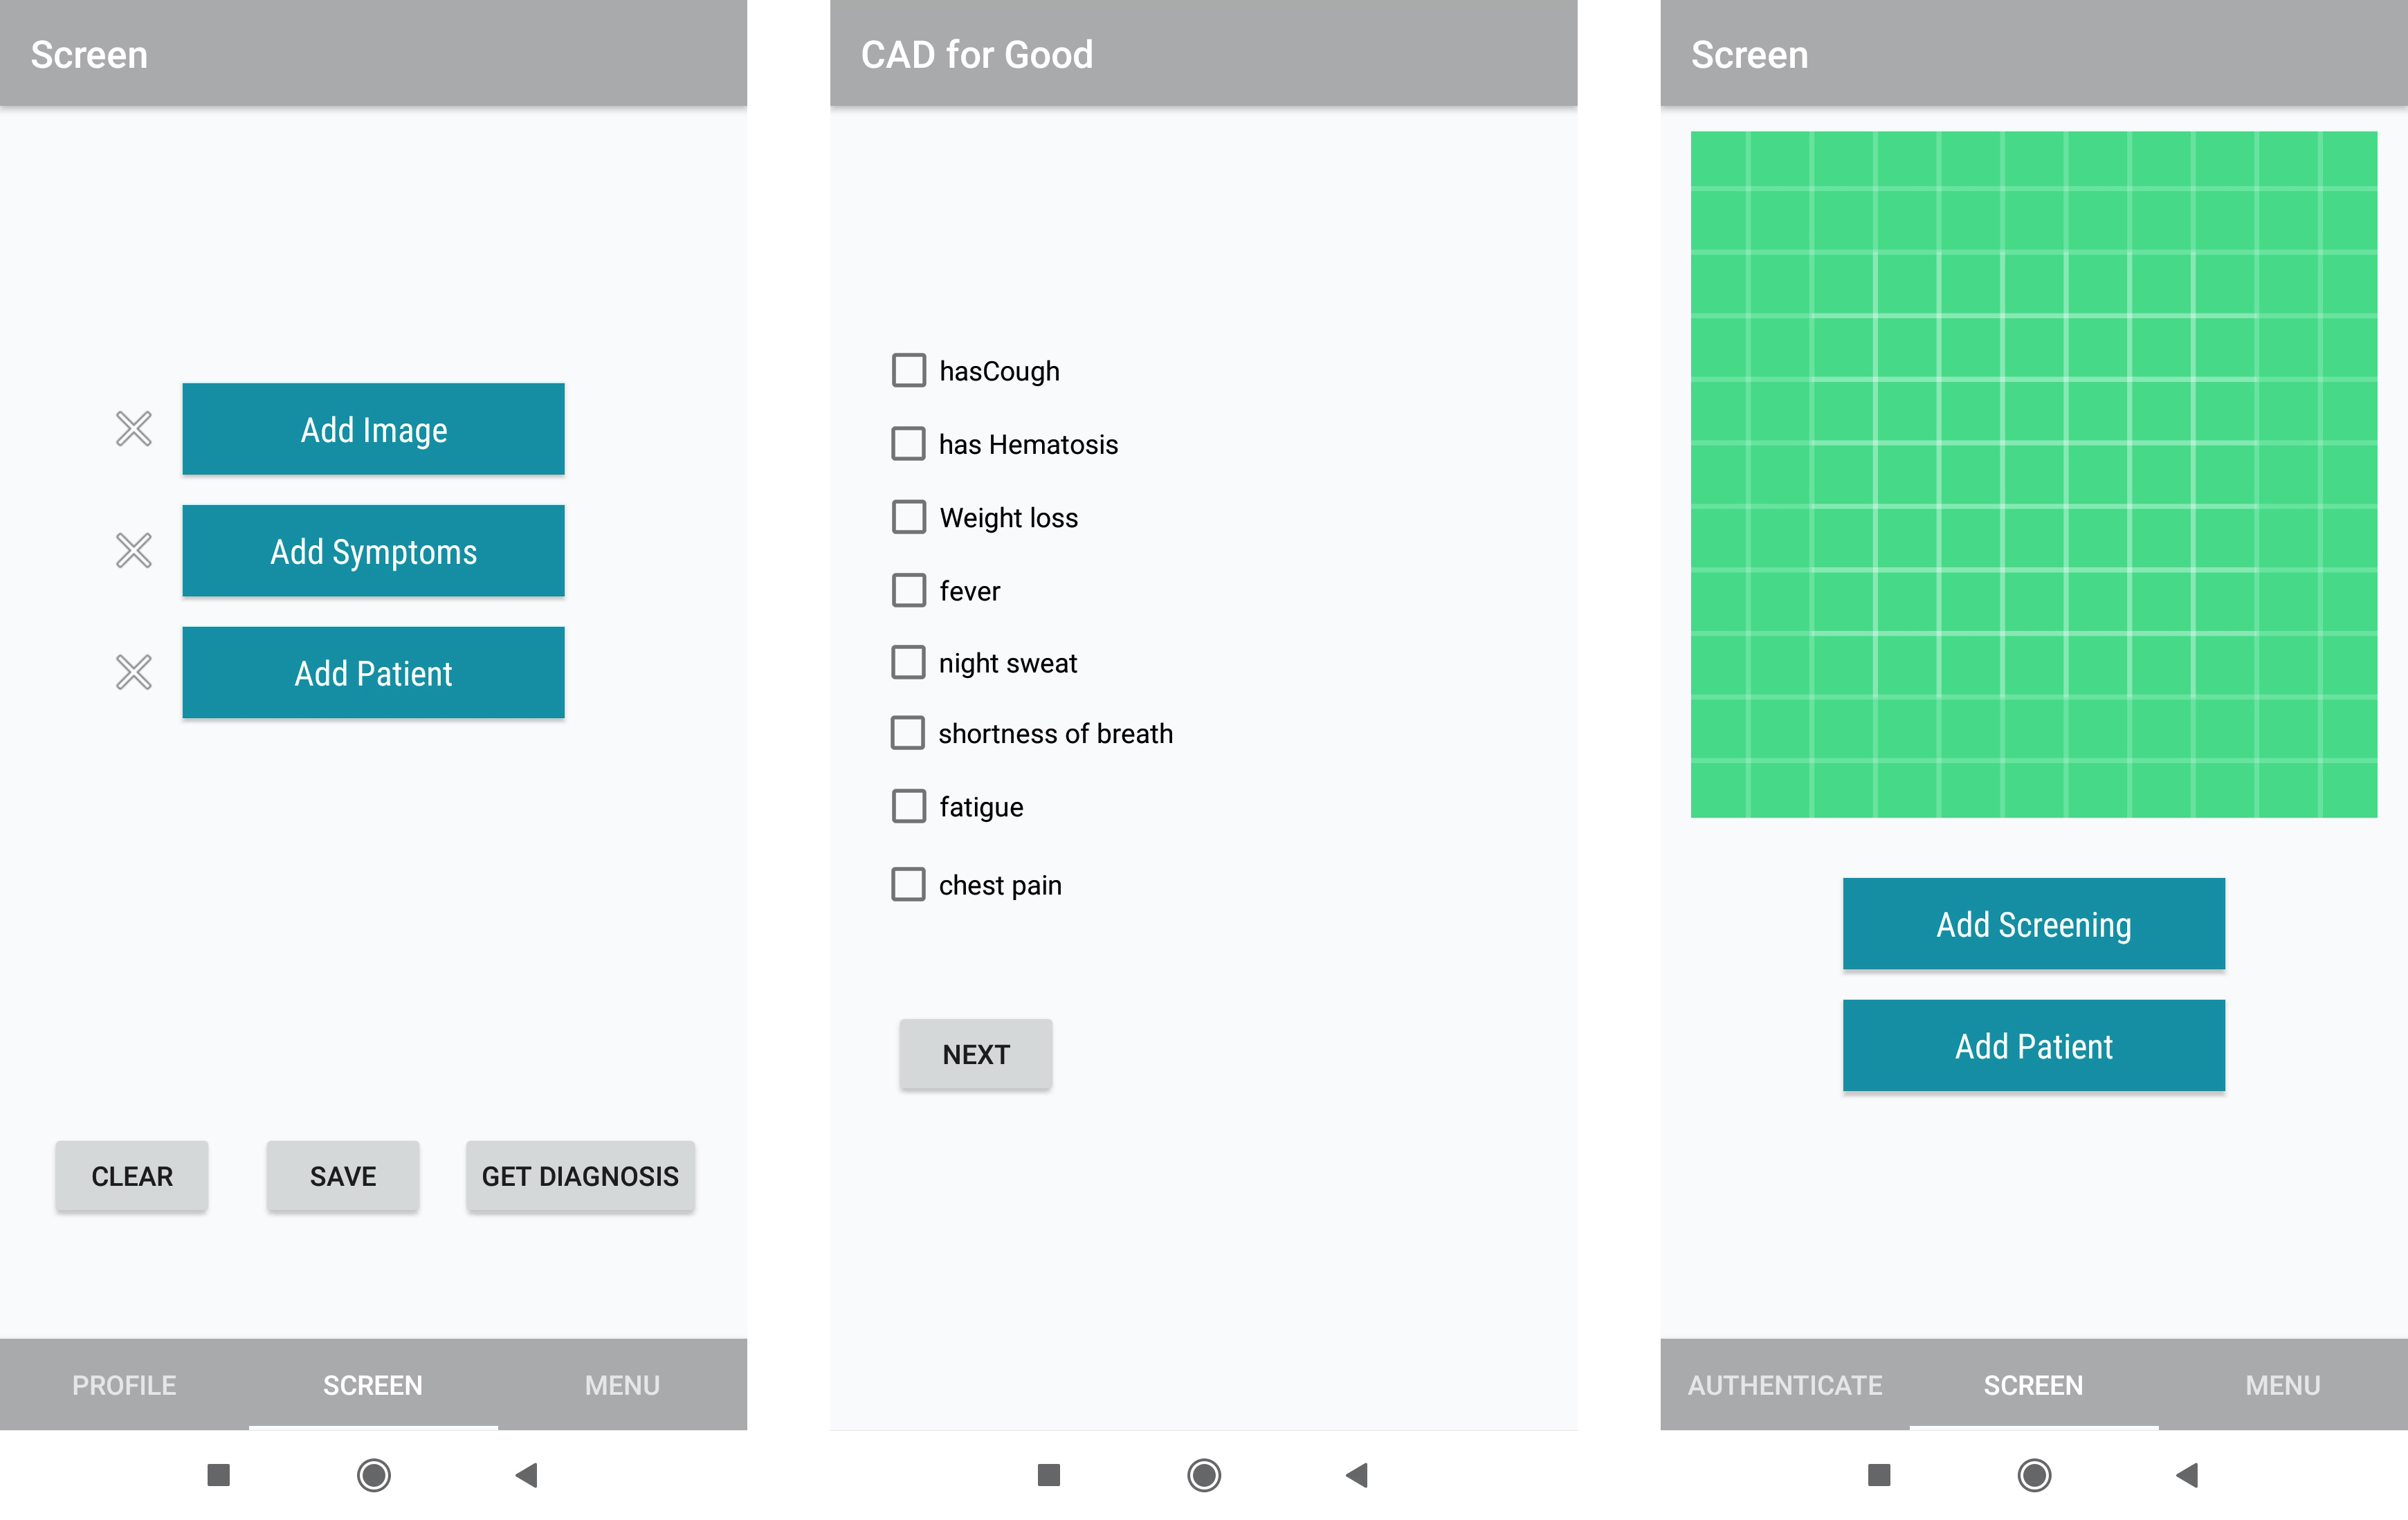
\includegraphics[width=1.0\linewidth]{pesti-report/images/android-client-screenshot-screen.jpg}
	\caption{Submit a screening using the Android app}
	\label{fig:android-client-screen}
\end{figure}
\\




\section{Tests}

We believe that we can only make sure that our code works if we test it. In this way, we have written unit tests for most of our API endpoints, where we would tests success cases and also error cases.
\\ \\
After some discussion about it, we decided to test only the back-end server and to not do front-end testing in our web and Android clients. We did't had the needed time to spend writting tests for all of our three components, so we decided to do it for the most important one, which was the back-end API. Below you can view a screenshot of some of the unit tests we wrote:


\\ \\
\begin{figure}[H]
	\centering
	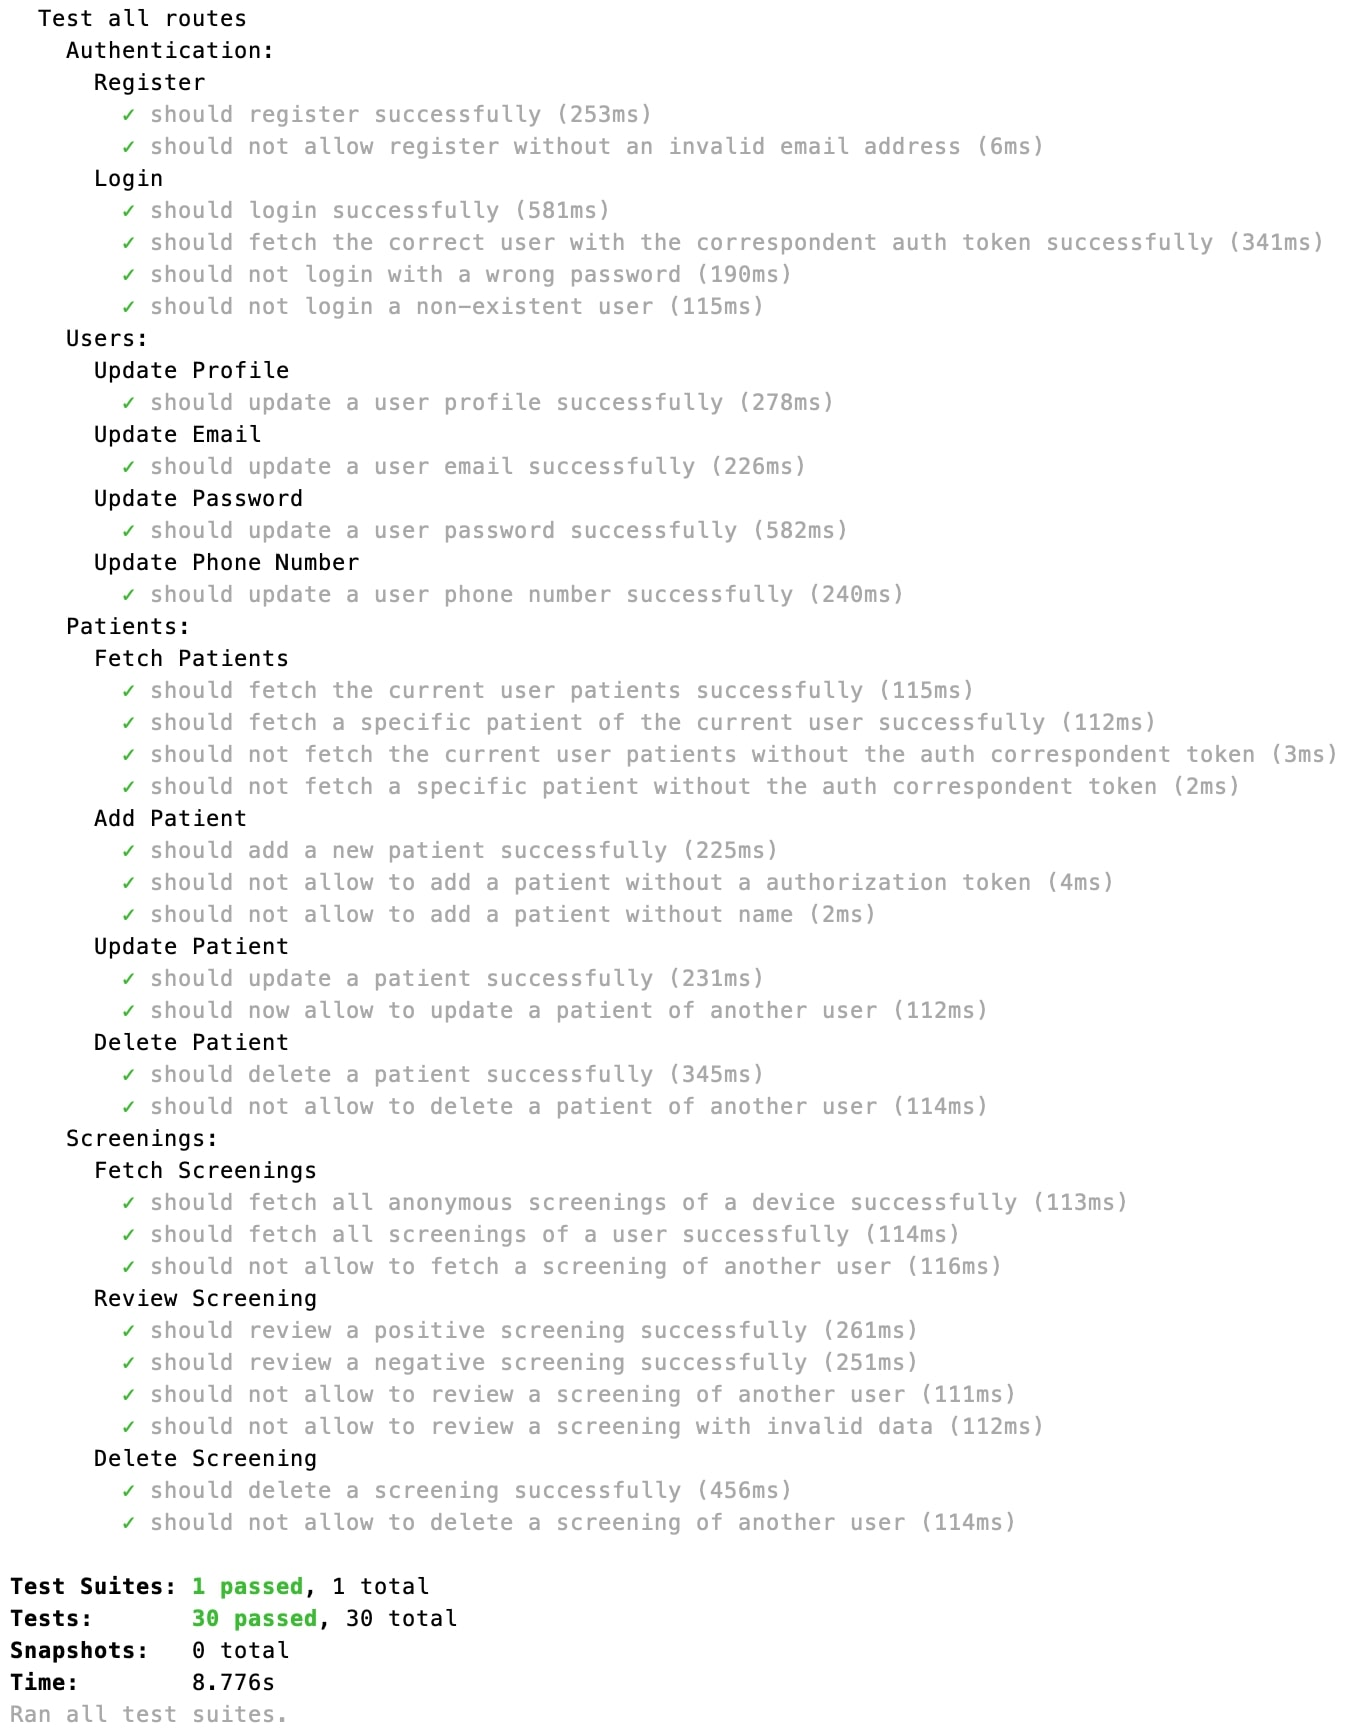
\includegraphics[width=1.0\linewidth]{pesti-report/images/unit-tests.jpg}
	\caption{Unit tests}
	\label{fig:unit-tests}
\end{figure}
\\

\section{Releases and deployment}

During our first face-to-face meeting in Belgium we decided that we would release and deploy the system as a whole and not the specific components (web client, mobile client and API). So instead of releasing by component we would release by feature, where we would develop the back-end and the front-end simultaneously.
\\ \\
We didn't agree on a fixed schedule of releases, so we would be releasing and documenting the changes every time we would feel that we had a good amount of issues delivered on that release. During our development time, we released three private alpha versions and a public open-source beta version. Below is our release management change-log:

\subsection{Version 0.1.0}

We released the alpha version 0.1.0 on 21 March 2020 with the following features:

\begin{itemize}

\item
Register
\item
Login
\item
Logout
\item
View the user profile
\item
Diagnose a screening
\item
View the screenings list
\item
View the details of a specific screening
\item
Add a patient
\item
View the patients list
\item
View the details of a specific patient
\item
View the about page
\item
View the privacy policy page

\end{itemize}

\subsection{Version 0.2.0}

Our second deployment, the alpha version 0.2.0 was released on the 8th of April of the same year with the following changes:

\begin{itemize}

\item
Edit the user profile (name, city, country and bio)
\item
Edit the user password
\item
Edit the user phone number
\item
Edit the user email address
\item
Reference a patient when diagnosing a screening
\item
View the output image of a screening
\item
Edit a patient details (name, sex and year of birth)
\item
View breadcrumbs for better navigation
\item
View the terms and conditions page
\item
View the cookie banner
\item
Multiple bug fixes

\end{itemize}

\subsection{Version 0.3.0}

Our third and last alpha deployment, the alpha version 0.3.0 was released on the 10 June 2020 with the following changes:

\begin{itemize}

\item
Send location data (latitude and longitude) when diagnosing a screening
\item
Properly view the diagnosis result of a screening
\item
Properly validate all input fields
\item
Refactored the style of the application
\item
Add contact page and form
\item
Multiple bug fixes

\end{itemize}

\subsection{Version 1.0.0}

Two days after our third release, on 12 June 2020, we released or first beta version 1.0.0, with some small bug fixes and deployed all our code on GitHub public as open source software using the MIT license.


\newpage\cleardoublepage

\chapter{Conclusion}
\section{Objectives achieved}

The objectives we set during our first meeting were mainly this three:

\begin{itemize}

\item
Build an RESTful API wrapper around EPCON's API with user authentication and persistent data
\item 
Build a web client with focus on user experience and performance
\item 
Build a mobile client with focus on user experience and performance

\end{itemize}

Our project was ambitious, we were 11 students from different countries and communicating in English (which for most of us, including myself, was not our native language), some more experienced than others in terms of working remotely, agile methodology and software development.
\\ \\
We successfully developed the REST API with persistent data and an authentication system and the two clients (web and Android). As of this moment, there are still bugs and issues to work on and the Android app was not yet released on the Google Play Store. Nevertheless, I think we mostly achieved the objectives we have defined at the beginning of the project.

\section{Limitations and future work}

During the execution and development of this project we have faced multiple challenges, some more with more impact than others. Here are some issues we have faced:

\begin{itemize}

\item
Cultural differences between team members
\item 
Working remotely on different time-zones
\item 
Experience gap in terms of agile software development

\end{itemize}

Most of the difficulties we faced were related to team-work issues. All of us were working remotely, in different countries, some in a very different time-zone which created barriers of communication. Another issue we faced was very different ranges of technical knowledge in software development tools and processes. Some of our team members were not familiar with popular programming languages like Java or JavaScript, others had not yet been introduced to versioning tools like Git and most were not familiar with the processes that software development takes, like writing user-stories, following a backlog and working following agile methods.
\\ \\
We have recently published all our code with a permissive open source license on GitHub. So, as of today anyone in the world can start contributing for the project. We plan on continuing to develop the system until September, where our main focus will be on finishing the Android app and bug fixing some issues on the server and on the web client.

\section{Final assessment}

Having the opportunity to work on this project was a pleasure for me. It strengthened my knowledge both in a technical perspective and a team-work related view. I've learned a lot about APIs and the Android SDK and working with such a culturally diverse team made me rethink on how much communication is important.
\\ \\
I feel that EPCON was appreciative of our work and recognized our efforts and in the end we effectively build a tool that was asked for us. Overall it was an amazing experience that I think everyone will take some knowledge home.
\newpage\cleardoublepage

% -------------------------------------------
% Bibliography

\renewcommand\bibname{Bibliography}
\addcontentsline{toc}{chapter}{Bibliography}
\bibliographystyle{IEEEtran}
\bibliography{bibliography/references}   


\end{document}

